\documentclass[12pt,letterpaper]{report}

% =============================================================================
% =  CUSTOM INFORMATION (stored as variables, used in template)
% =============================================================================

% The title of the paper.
\newcommand{\paperTitle}{Structural Quality \& Software Evolution}

% The name of the author.
\newcommand{\paperAuthor}{Alison Major}

% The author's concentration in their Master of Science in Computer Science
\newcommand{\authorConcentration}{Software Engineering}

% =============================================================================
% =  PREAMBLE (packages and custom code)
% =============================================================================

\usepackage{paperPreamble}

% =============================================================================
% =  BEGINNING OF THE DOCUMENT
% =============================================================================

\begin{document}

% Include Page Numbers - Roman Numerals for Front Matter
\cleardoublepage% \clearpage
\pagenumbering{roman}
\pagestyle{plain}

% =============================================================================
% =  Paper Title & Author Information
% =============================================================================

\begin{titlepage}
  \begin{center}
    
    \vfill
    
\includegraphics[width=0.8\textwidth]{UniversityLogo}
    
    \vspace{3cm}
    \large
    \textbf{\paperTitle}

    \vspace{0.5cm}
    A Thesis

    \vspace{0.5cm}
    By

    \vspace{0.5cm}
    \textbf{\paperAuthor}

    \vspace{2cm}
    Department of Computer and Mathematical Sciences

    \vspace{0.5cm}
    Submitted in partial fulfillment of the requirements

    \vspace{0.5cm}
    for the degree of \\
    Master of Science in Computer Science, 

    \vspace{0.5cm}
    Concentration in \authorConcentration

    \vspace{2cm}
    \today
          
  \end{center}
\end{titlepage}


% Set the document to be double spaced 
% http://kb.mit.edu/confluence/pages/viewpage.action?pageId=3907092
\doublespacing

% =============================================================================
% =  Signature Page
% =============================================================================

\newpage
\noindent
The undersigned have examined the thesis entitled `\textbf{\paperTitle}' presented by \textbf{\paperAuthor}, a candidate for the degree of \textbf{Master of Science in Computer Science (Concentration in \authorConcentration)} and hereby certify that it is worthy of acceptance.

\begin{center}
  \begin{tabularx}{1\textwidth} {
    >{\raggedright\arraybackslash}X
    m{1cm}
    m{3cm}
  }
    & & \\ & & \\ % Empty rows for spacing
    \cline{1-1} \cline{3-3}
    Advisor & & Date \\
    
    & & \\ & & \\ % Empty rows for spacing
    \cline{1-1} \cline{3-3}
    Program Director & & Date \\
    
    & & \\ & & \\ % Empty rows for spacing
    \cline{1-1} \cline{3-3}
    Department Chair & & Date 
  \end{tabularx}
\end{center}


% =============================================================================
% =  Paper Abstract
% =============================================================================

\newpage
\addcontentsline{toc}{section}{Abstract}
\section*{Abstract} \label{sectionAbstract}

% State the problem.
Some software engineering projects fail to evolve, which makes them obsolete.
% Say why this problem is interesting.
This topic is interesting and important to developers because the software that fails to evolve will fail to generate user engagement, leading to revenue loss.
% Say what my solution achieves.
We review a number of projects and resources to understand the correlation of software structure quality and its impacts on a system's ability to evolve.
% Say what follows from my solution.
With this understanding, we explore ways to improve the evolution of a software system through tools and suggestions.

% When writing an abstract, bare in mind an abstract is a short descriptive summary of your thesis. The number of words accepted might vary e.g. 200-250 words. An MS thesis abstract need not exceed two pages. Abstracts are typically written last although they are the most important part of the thesis. They should have a little bit of everything: the background, the scope of your project, the purpose, findings and conclusions. An abstract is neither paragraphed nor cited. It should not be written as a literature review or a discussion of results. In a simplistic manner, your abstract, in a few words, should answer the questions: why should we care about your research; how did you get your results; what did you learn, find, create, invent; and finally what do your results imply?


% =============================================================================
% =  Acknowledgements
% =============================================================================

\newpage
\addcontentsline{toc}{section}{Acknowledgements}
\section*{Acknowledgements} \label{sectionAcknowledgements}

This research and working towards my degree has been an endeavor and one that I would not dream of tackling on my own.

First, my thanks go to God, the ultimate creator, who formed us all to be creators fitting our skills. And to His son, Jesus, who gave his life so that the sins of the world may be forgiven, and rose from the dead and now sits at the right hand of God.

Second, much gratitude goes to my very creative and patient family. I am thankful for my husband, Chris, who was foundational in finding the time and focus on working on my studies. My amazing kids, Ewan and Gwynnie, have provided patience, encouragement, and numerous trips to the library. I could not have gotten through this without all of your support.

Finally, I am grateful for my coworkers and my professors. The Robotic Process Automation (RPA) team at Sysco has been cheering me on from the sidelines. The professors at Lewis University have provided mentorship and guidance. They have all encouraged me as I've worked to apply my knowledge from the last decade of my experience as a software developer and gather new information that has helped us build better software solutions.


% =============================================================================
% =  Table of Contents
% =============================================================================

\newpage
\begin{singlespace}
  \tableofcontents
\end{singlespace}

% =============================================================================
% =  List of Tables
% =============================================================================

\newpage
\addcontentsline{toc}{section}{List of Tables}
\begin{singlespace}
  \listoftables
\end{singlespace}

% =============================================================================
% =  List of Figures
% =============================================================================

\newpage
\addcontentsline{toc}{section}{List of Figures}
\begin{singlespace}
  \listoffigures
\end{singlespace}

% =============================================================================
% =  Paper Content
% =============================================================================

% Include Page Numbers - Numbers (Arabic) for Main Matter
\cleardoublepage% \clearpage
\pagenumbering{arabic}

% \todo{========== INSERT SOMEWHERE ==========} 

% \begin{figure}[ht]
%   \centerline{
%     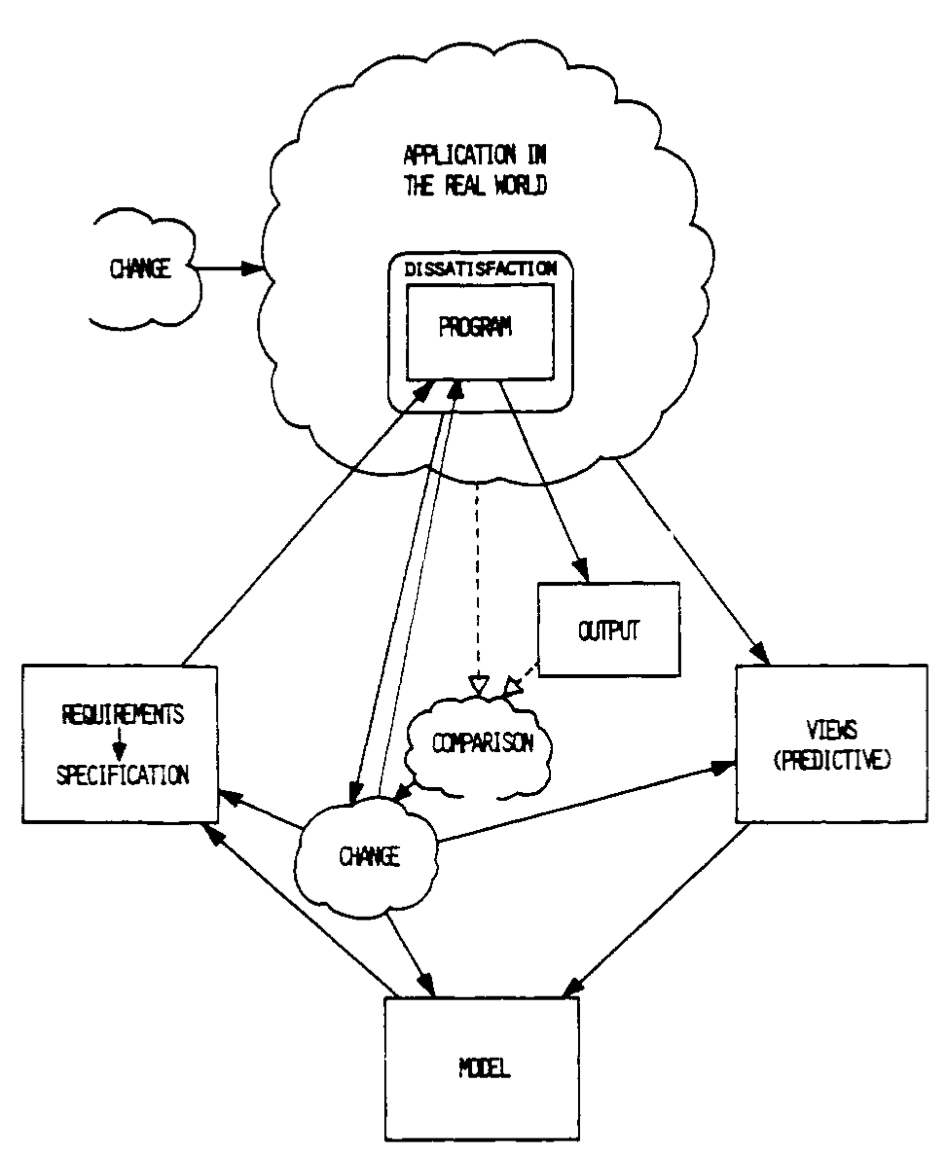
\includegraphics[width=0.7\columnwidth]{Lehman_Figure4.png}
%   }
%   \caption{Lehman's depiction of ``E-Programs'' \cite{lehman:1980}}
%   \label{figEPrograms}
% \end{figure}

% The programs we write become part of the world around that it models. These programs, especially with the advent of mobile technology, have become embedded in our world. Lehman recognized this decades ago and acknowledged the relationship of these types of programs to our world, as seen in Fig. \ref{figEPrograms}. \cite{lehman:1980}

% ``Software Maintainability is an indispensable factor to acclaim for the quality of particular software. It describes the ease to perform several maintenance activities to make a software adaptable to the modified environment. The availability \& growing popularity of a wide range of Machine Learning (ML) algorithms for data analysis further provides the motivation for predicting this maintainability.'' \cite{gupta:2021}

% ``This study would open new doors for the software developers for carrying out comparatively more precise predictions well in time and hence reduce the overall maintenance costs.'' \cite{gupta:2021}

% ``There are ten software maintainability measurements used in selected primary studies: CHANGE maintenance effort, corrective maintenance, adaptive maintenance effort, maintenance evaluation by maintainability index, maintenance evaluation by change proneness, maintenance time, maintenance cost, maintenance attributes, maintenance components and other measurements.'' \cite{alsolai:2019}

% There have been studies done to help visualize the evolution of software through the use of city maps. \cite{steinbruckner:2012}

% The EvoStreets approach follows 3 models to build up the map \cite{steinbruckner:2012}:
% \begin{enumerate}
%   \item The \textbf{primary model} for software cities captures structural and analysis data.
%   \begin{itemize}
%     \item Structural data refer to the static software structure, i.e. the decomposition into subsystems and modules, as well as dependencies among modules.
%   \end{itemize}
%   \item The secondary model is a 2.5D \textbf{geometric model}, representing primary model data
%   \begin{itemize}
%     \item captures the main structural and evolutionary properties of the software system
%     \item provides a specific, stable gestalt for each software system
%     \item --mainly influenced by the particular layout of the system elements
%   \end{itemize}
%   \item \textbf{Thematic tertiary models}
%   \begin{itemize}
%     \item designed to support specific application scenarios by visualizing particular aspects of a given software system and its development history
%   \end{itemize}
% \end{enumerate}

% ``Software process improvement (SPI) is seen as the dominant approach to improving software products in software development organisations [1].'' \cite{herranz:2019}

% % [1] --> Shih, C.-C., Huang, S.-J.: ‘Exploring the relationship between organizational culture and software process improvement deployment’, Inf. Manage., 2010, 47, (5–6), pp. 271–281

% ``SPI has become the primary approach to improving software quality and reliability, employee and customer satisfaction, and return on investment [2].'' \cite{herranz:2019}

% % [2] --> Mathiassen, L., Ngwenyama, O.K., Aaen, I.: ‘Managing change in software process improvement’, IEEE Softw.., 2005, 22, (6), pp. 84–91

% ``The result of this study shows that maintainability is the most significant and ubiquitous product quality characteristic considered in the literature while usability is the most significant attribute in the quality in use category.'' \cite{adewumi:2016}

% \todo{========== END THINGS TO INSERT ==========}

% Chapter one defines the overall importance of the problem areas and provides an introduction into what you did.
\newpage
\chapter{Introduction} \label{sectionIntroduction}

When building software systems, we have several areas of concern: cost, delivery timeline, quality, etc. The cost and time-to-market are often the two problems given the highest priority in a project. However, engineers must consider the software quality to preserve the system's longevity. Despite its importance, the code and architecture quality can be challenging to understand and measure.

The art of programming began as something very tedious and error prone, with programmers writing every step of a process in a machine language. As this was not a great way to grow the industry, languages were developed so that programmers could reduce the manual effort of their programming and also improve the quality of their work by allowing the machine itself to transform the high-level code into something executable and efficient. \cite{lehman:1980}

With the creation of programming languages, the ability to build systems and applications has become a skill that most anyone can learn. Open source project create communities of learning and advancement. However, all systems need structure and an investment of time.

When we think about projects, we can assume that as time goes on and changes and additions occur within a system's source code, the complexity of that system will grow. However, when we manage the code structure, we can keep the complexity in check, allowing systems to evolve. Developers can maintain this structure through simple steps like having readable code and more complex considerations, like how coupled and cohesive a system is.

One way to understand the quality around a system is to discuss its ``maintainability,'' the ease of receiving new features or resolving bugs. For example, developers may find that adjusting one area to add a new feature requires touching several other code areas in tightly coupled systems. Some code measuring systems provide a Maintainability Index (MI), a well-known quality measure. While the effectiveness in quantifying software quality is debated, many quality models include MI measurements \cite{vandeursen:2014}, \cite{adewumi:2016}. 

Adewumi et. al found that maintainability is measured by 55\% of the existing Open Source Software (OSS) quality models, making it the most common quality characteristic measured \cite{adewumi:2016}. From ``Fig.~\ref{figFreqDistProductQualityModel}'', we can infer that maintainability is more important than functional stability. If the code is maintainable and accessible, missing features can be incorporated, but if it is difficult to read and understand and is not well documented, those missing features would be hard to implement \cite{adewumi:2016}.

\begin{figure}[ht]
  \centerline{
      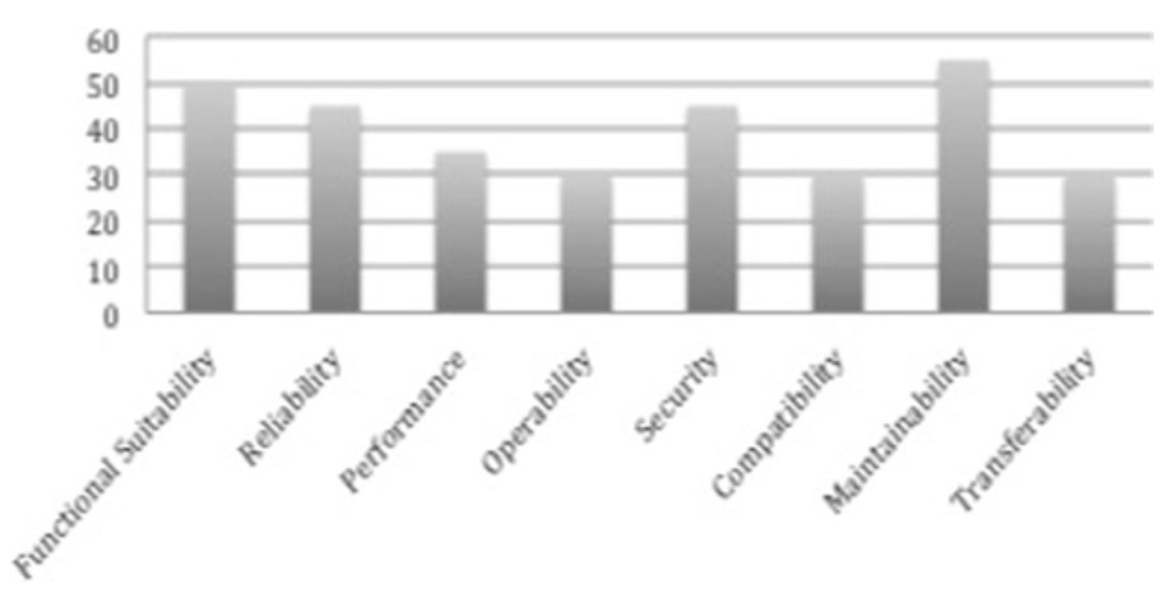
\includegraphics[width=0.7\columnwidth]{adewole_ProductQualityCharacteristics_in_OSS_quality_models.png}
  }
  \caption{Frequency distribution of ISO 25010 product quality characteristics in OSS quality models, as found by Adewumi et. al in 2016 \cite{adewumi:2016}.}
  \label{figFreqDistProductQualityModel}
\end{figure}

Code smells are used extensively by practitioners to identify low-quality spots in the software system. These areas would need the teams' attention and are good candidates for refactoring. Rather than putting focus on building comprehensive models with all possible software characteristics, developers should instead focus on the essential characteristics: maintainability, usability, and maintenance capacity of a software community \cite{adewumi:2016}.

% \todo{TODO: Consider analogy of how Blockbuster did not evolve and eventually closed.}

\section{Maintainability Index \& Refactor Scores}

``Software maintainability is one of the fundamental external quality attributes and is recognised as a research area of primary concern in software engineering \cite{alsolai:2019}.'' As such, we need to find ways to measure the maintainability of a software system. As mentioned earlier, many OSS quality models already include maintainability as a characteristic measurement.

Pylint is a static analysis tool that identifies several classes of code quality concerns. Refactor violations are relevant to our study, which reports various code smells. However, we can assume there must be some correlation between the Maintainability Index and the type and number of code smells in a software system, quantified by the Pylint refactor score.

To compute various code metrics, Radon is another Python tool available \cite{radon:docs}. One such score that Radon provides is the Maintainability Index (MI), which tells us how easy it should be to support and change the program. Radon calculates this value using a formula that consists of SLOC (Source Lines Of Code), Cyclomatic Complexity, and Halstead volume.

This study explores such assumptions and systematically investigates any correlation between Radon's Maintainability Index metric and the Pylint Refactor message count. Furthermore, we perform analysis on specific refactor violations to reveal and shed light on the relative effectiveness of the different refactor violations and their relationship to Maintainability Index.

The structural quality of a software system will impact the software evolution. If the project has poor structural quality, the architecture will minimize its ability to evolve, and the software system will eventually ``die off'' so to speak.

We will look at many open-source Python systems using Pylint and Radon and attempt to correlate the data from the scores to the level of ease in adding new features to the system. The Pylint and Radon results will determine if a system is more maintainable with better scores.

\section{Paper Structure}

% Chapter 2: Background & Literature Review    \ref{chapterBackground}
% 2.1 - Keeping users engaged long term        \ref{sectionTheProblem}
% 2.1.1 - Why software evolution matters
% 2.1.2 - How do we ensure software evolution
% 2.2 - The impact of structural quality       \ref{sectionMyIdea}
% 2.2.1 - Software maintenance
% 2.2.2 - Software evolution
% 2.2.3 - Measuring maintainability
% 2.2.4 - Maintainability scores
% 2.2.5 - Other maintainability characteristics
% 2.2.6 - Documentation and maintainability
% 2.4 - Related Work                           \ref{sectionRelatedWork}

In Chapter \ref{chapterBackground}, we will dig into a deeper background of the topic, exploring ideas of why software systems need to keep users engaged long term (Section \ref{sectionTheProblem}). We will explore automated measurements that provide evaluation scores of software systems. By using some of these quality and maintainability scores, we can see how structure impacts evolution (Section \ref{sectionMyIdea}). Additionally, we'll explain how maintainability is measured, as well as the difference attributes that can factor into maintainability. We will also review related works (Section \ref{sectionRelatedWork}).

% Chapter 3: Methodology                       \ref{chapterMethodology}
% 3.1 - Initial repository set                 \ref{sectionInitialSet}
% 3.2 - Filtered repository set                \ref{sectionFilteredSet}

With more background on the problem, we can then review the methodology for our research in Chapter \ref{chapterMethodology}. Here we will review where we found our initial data set (Section \ref{sectionInitialSet}) and what criteria we used to filter it to a manageable size for our tests (Section \ref{sectionFilteredSet}).

% Chapter 4: Results                           \ref{chapterResults}

Chapter \ref{chapterResults} will review the results of our research, using the methodology previously explained.

% Chapter 5: Conclusions and Recommendations   \ref{chapterConclusion}

We will then provide final conclusions and recommendations in Chapter \ref{chapterConclusion}.


% Chapter two is why you did it in the context of what was previously known.
\newpage
\chapter{Background and Literature Review} \label{chapterBackground}

\todo{TODO: Chapter 2 - why I did it in the context of what was previously known}

The background and literature review section needs to provide sufficient fundamental background information about the subject to support your objectives, hypothesis (or research questions) and methods, and review the pertinent literature related to the specific problem / hypothesis you are addressing. In Johnson (1991), some of the questions that he listed that the literature review should be to answer include: 

\begin{itemize}  
	\item what are the fundamental science, math, engineering concepts related to your research (scope),
	\item what part of your research work has ever been investigated before and what has not, (some of this may have been included in the introduction)
	\item how does your research work relate to that done by others, 
	\item how have others defined/measured/identified the key concepts of your research, 
	\item what data sources have you used or have other researchers used in developing general explanations for observed variations in a behavior or phenomenon in a concept in your thesis etc.  
\end{itemize}

The lit review (~20 pages or more) should not be limited to the above questions only. Ingeniousness and creativity is expected of a grad student.
Bullets can be single spaced.  The above bullets are in the style “thesis-bullets.”  When you type bulleted text, highlight the bulleted text and then select “thesis-bullets” from under the format, style menu to automatically change their formatting as above.

% include the section
\section{Section header}

Given the length of each chapter, it is required to use headers and sub headers (possibly sub-sub headers).  These can be numbered or one can just rely on different formats.  The section headers in this document are labeled “heading 2” (“heading 1” was used for chapter titles).  The heading styles formats should be consistent throughout the document as it helps significantly in creating the automatic table of contents.

\subsection{Sub Heading}

The subheadings here have a different format (“heading 3”) than the section headers.

\subsubsection{Sub-Sub Heading}

You can even get to another level of headers, defined here as “heading 4.”  The table of contents, however, is currently set up to just include three levels of headers.

\subsection{Equations}

Equations can be created in MS WORD equation editor or they can be created with other software.  Equations should be numbered.  They can be numbered within each chapter (e.g., 2.1, 2.2) or they can be numbered sequentially throughout the entire thesis.  Equations should be indented or centered with the equation number to the right.  The example below and associated “thesis-eqn” style can be used for all your equations.

\todo{Include example of an equation here.}

This equation was written with the equation editor. Found through “insert, object, equation editor 3.0. The equation editor can also be found through “tools, customize, commands”, and in categories, look for insert and in the commands section, look for equation editor, drag and drop the icon onto the toolbar. This editor is fine for relatively simple equations, other options are available for more complex equations.

\subsection{Tables}

Tables should have meaningful information with descriptive headers.  You can use the “thesis-table caption” style to define your captions and refer to the table in the text with a “cross reference” (Table 1).  MS Word re-numbers table captions automatically when new tables inserted.  But you need to right click on any cross references and “update field” if there are changes.

\begin{table}[h!]
  \centering
  \begin{tabularx}{0.8\textwidth} {
    | >{\centering\arraybackslash}X 
    | >{\centering\arraybackslash}X 
    | >{\centering\arraybackslash}X |
  }
    \hline
      Step \# & Instruction \\ 
    \hline
      Create table caption & Insert, reference, caption, table \\ 
    \hline
      Format the caption & Format, style, “thesis-table-caption” \\ 
    \hline
      Create table & Table, insert… \\
    \hline
      Format the table & The formatting of the table can vary, including use of single space as appropriate. Most journals require that tables are formatted using table style “Table Simple 1” format. \\
    \hline
      Reference the table from text & With the cursor at the location you want to cite the table: insert, reference, cross reference, table, label and number only. \\
    \hline
  \end{tabularx}
  \caption{Table 1: Steps in creating a table}
  \label{table:1}
\end{table}

\subsection{Figures}

Figures and illustrations are a necessary means of communicating technical information.  Often times, figures included in the background/lit review section are copied from existing copyrighted information.  In all cases, this is technically inappropriate without also receiving permission from the copyright owner.  Citing the source of the figure is not sufficient. This rule is enforced for PhD dissertations because they are submitted to ProQuest for electronic access by others.  The enforcement of this rule for MS theses is dependent on the specific committee members.

Resolution of figures is often a problem in theses.  Resolution should be >300 dpi, preferably 600dpi (\ref{fig:figure1}).  You should note that saving images as jpeg files is a sure way to lower the resolution to an unacceptable extent.  From experience, a good way is to copy your graphic (for example from PowerPoint or excel) and when pasting it into word, use the “paste special” “as an “enhanced metafile” (\ref{fig:figure2}).  This also substantially reduces the resulting file size in comparison with pasting graphs in as excel graphics.

\begin{figure}
  \centering
  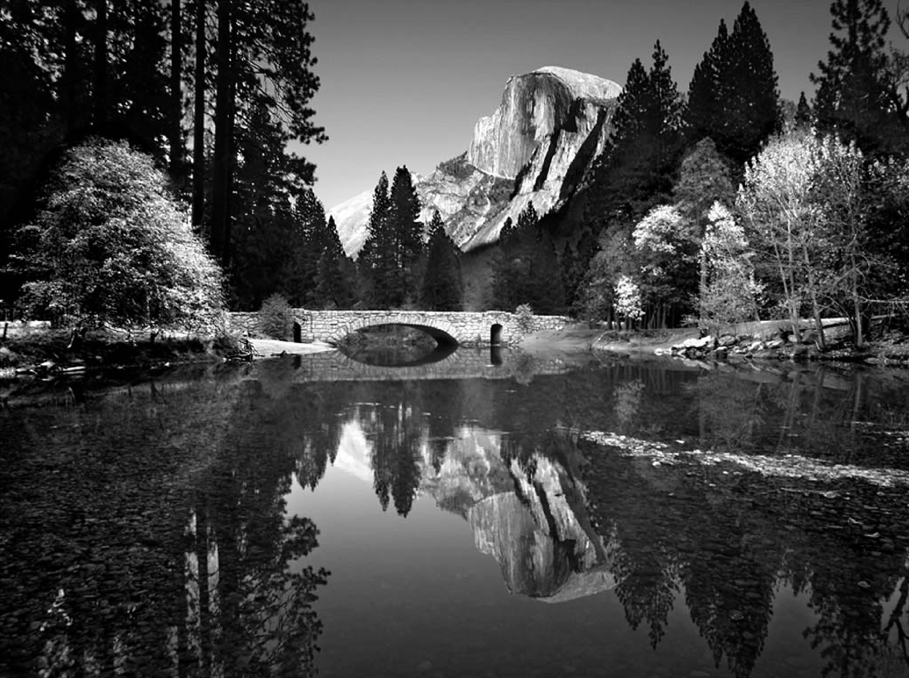
\includegraphics[width=0.8\textwidth]{Figure1}
  \caption{Figure 1: Example photo with high resolution.  Caption created with ``insert, reference, caption, figure'' and the style changed to ``thesis-figure caption.''}
  \label{fig:figure1}
\end{figure}

\begin{figure}
  \centering
  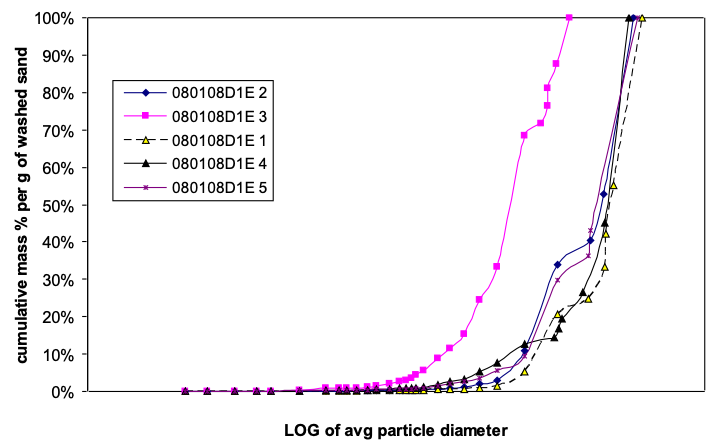
\includegraphics[width=0.8\textwidth]{Figure2}
  \caption{``Figure 2: Example of high resolution graphic inserted with “paste special, as enhanced metafile''}
  \label{fig:figure2}
\end{figure}


Sub heading (heading 3)
The subheadings here have a different format (“heading 3”) than the section headers.

Sub-sub heading (heading 4)
You can even get to another level of headers, defined here as “heading 4.”  The table of contents, however, is currently set up to just include three levels of headers.

Equations
Equations can be created in MS WORD equation editor or they can be created with other software.  Equations should be numbered.  They can be numbered within each chapter (e.g., 2.1, 2.2) or they can be numbered sequentially throughout the entire thesis.  Equations should be indented or centered with the equation number to the right.  The example below and associated “thesis-eqn” style can be used for all your equations.
		[1]
This equation was written with the equation editor. Found through “insert, object, equation editor 3.0. The equation editor can also be found through “tools, customize, commands”, and in categories, look for insert and in the commands section, look for equation editor, drag and drop the icon onto the toolbar. This editor is fine for relatively simple equations, other options are available for more complex equations.

Tables
Tables should have meaningful information with descriptive headers.  You can use the “thesis-table caption” style to define your captions and refer to the table in the text with a “cross reference” (Table 1).  MS Word re-numbers table captions automatically when new tables inserted.  But you need to right click on any cross references and “update field” if there are changes.
Table 1: Steps in creating a table

Figures
Figures and illustrations are a necessary means of communicating technical information.  Often times, figures included in the background/lit review section are copied from existing copyrighted information.  In all cases, this is technically inappropriate without also receiving permission from the copyright owner.  Citing the source of the figure is not sufficient. This rule is enforced for PhD dissertations because they are submitted to ProQuest for electronic access by others.  The enforcement of this rule for MS theses is dependent on the specific committee members.
Resolution of figures is often a problem in theses.  Resolution should be >300 dpi, preferably 600dpi (Figure 1).  You should note that saving images as jpeg files is a sure way to lower the resolution to an unacceptable extent.  From experience, a good way is to copy your graphic (for example from PowerPoint or excel) and when pasting it into word, use the “paste special” “as an “enhanced metafile” (Figure 2).  This also substantially reduces the resulting file size in comparison with pasting graphs in as excel graphics.

Figure 1: Example photo with high resolution.  Caption created with “insert, reference, caption, figure” and the style changed to “thesis-figure caption.”



Figure 2: Example of high resolution graphic inserted with “paste special, as enhanced metafile”
% =============================================================================
% =  The Problem (1 page)
% =============================================================================

\section{Keeping Users Engaged Long Term} \label{sectionTheProblem}

% --- The problem is that some projects fail to evolve ------------------------

When developing a new system or a new software idea, getting the project off the ground and in front of users is one thing. However, keeping that project alive with a thriving community of engaged users is another.

The systems we create could be customer-facing web applications, games, or internal applications used to carry out tasks. Regardless of the type of system, the product will no longer provide usefulness without evolving with the user's needs. Even in a corporate setting with internal business systems, over time, users will need change; how a system can adapt to those needs requires a level of flexibility.

\vspace{0.25cm}
\begin{displayquote}
``Software evolution is the continual development of software after its initial release to address changing stakeholder and/or market requirements.'' \cite{wiki:software-evolution}
\end{displayquote}
\vspace{0.25cm}

% --- Why does it matter if a project does not evolve? ------------------------
\subsection{Why does software evolution matter?}

When a system cannot evolve, the impact is primarily felt by the users. However, this impact will eventually get back to those who created and continue to support the system. With users that are either unsatisfied or unable to use the system any longer, the engagement levels will drop. The decline in users will ultimately result in a loss of income, as the system can no longer deliver to the needs of its audience.

Because organizations invest large amounts of money in the software systems that they create, they depend on the software's continued success. Software evolution will allow the system to adapt to new or changing business requirements, fix bugs and defects, and integrate with other systems that have changed and evolved that may share the same software environment.

As a system is used, inevitably, users will stumble into situations that even the best quality assurance testers will miss. When defects are found, they will require fixing. 

To keep a system up-to-date, we must add new features. For example, there may be a need to improve a system's performance or reliability, especially if the user base expands.

Security can also impact the need for a system to be maintained. New ways to infiltrate a system can be uncovered, so it is important to stay on top of newest versions of dependencies and technologies in order to avoid potential breaches of data and experience.

% --- How do we ensure a project will be able to evolve? ----------------------
\subsection{How do we ensure software evolution?}

Because the maintainability of a system can ultimately influence the ability to generate revenue, we must find ways to ensure that a project will evolve. One of these ways could be to ensure that a project continues to be considered ``maintainable'' throughout its lifetime. This system characteristic will ensure that bugs can be fixed quickly, but new features should be easy to add as the users' needs evolve.

% =============================================================================
% =  My Idea (2 pages)
% =============================================================================

\section{The Impact of Structural Quality} \label{sectionMyIdea}

% --- Understand Software Maintenance -----------------------------------------
\subsection{Software Maintenance} \label{subSoftwareMaintenance}

The structural quality of a software system will impact the software evolution. Similarly, as a project evolves, it is likely to degrade, as developers often make changes quickly and in ways that the original design did not anticipate \cite{martin:2000}. However, if the project has poor structural quality, its ability to evolve will be minimized, and the software system will eventually ``die off.''

There is much planning involved in all software creation projects in what the product will be, will do, who it is for, and so on. One of the things that should also be on the planning list is long-term maintenance and growth. So how do we build a thing that will be easier to add features to down the road?

Let us define maintainability in the context of software. For example, it would be easy to maintain if a system is easy to debug and easy to add new features. These new features are generally considered minor features and may often be reported as bugs by users when, in reality, they are looking for functionality enhancements \cite{wiki:software-maintenance}.

\vspace{0.25cm}
\begin{displayquote}
  ``Software maintenance in software engineering is the modification of a software product after delivery to correct faults, to improve performance or other attributes.'' \cite{wiki:software-maintenance}
\end{displayquote}
\vspace{0.25cm}

It may be easier to understand what characteristics define a system with poor maintainability. These types of systems will have poor code quality, leading to defects. For instance, there could be undetected vulnerabilities or exposures, or it may be that the system is overly complex. In addition to the complexity, it could be hard to read due to the poor naming of dead (unused) code throughout the source code.

A project is known to have good maintainability when there is an enforced set of clean and consistent standards for the code. These standards often involve having human-readable names for functions, methods, and variables. Minimize any complex code and methods should be small and focus on a single thing. Parts of the system are decoupled and organized, making it easy to work on different parts with low impact on unrelated parts. In other words, the code is DRY (\underline{D}on't \underline{R}epeat \underline{Y}ourself \textemdash there is limited redundancy in the code), unused code has been removed, and there is a level of documentation that supports an easy understanding of the system.

% \todo{TODO: Anything about SOLID and when too many files are being touched? \cite{martin:2000}}

Why should we care about whether the code is maintainable? There is an assumption that the majority of cost over the lifetime of a project falls under maintainability. Fred Brooks, in his book ``The Mythical Man-Month'' (1975), even claimed that over 90\% of the costs for a typical software system come up in the maintenance phase \cite{brooks:mythical}. In 1977, Meir M. Lehman noted that maintenance accounts for 70\% of a program budget, with 30\% spent on development. In 1993, there was another observation that the development of a typical project uses only 20-40\% of the resources (money, time, effort), with 60-70\% used for maintenance activities \cite{ieee:1219}.

Once the bulk of the system is off the ground and live worldwide, how well the team can improve the system with new features and fix bugs, even working on different parts in parallel, can be impacted by its maintainability. Any successful piece of software will inevitably need to be maintained.

% --- Understand Software Evolution -------------------------------------------
\subsection{Software Evolution} \label{subSoftwareEvolution}

There is a distinction to be made between \textbf{software maintenance} and \textbf{software evolution}. From here, we will refer to software maintenance as bug resolution and minor functional improvements. In other words, we can consider this routine maintenance when we must fix a broken route in the application or provide a subtle enhancement to the user experience. In contrast, when we look at upgrades, adaptations to the changing and growing needs of the user, or migrating the system to new technology, we can refer to this as the evolution of the software.

The evolution of software can result from new laws that have come into being. As technology changes, governing bodies must continually revisit data collection and information sharing policies. As a result, changes in technology and laws may lead to adaptations in the software systems.

It is also fair to say that systems will change because we can never fully determine a user's needs at the start of a project. Thus, it would be safe to say that users' needs will change over time. However, the changing user needs can lead to a never-ending project that will always need some form of enhancement.

Meir ``Manny'' Lehman and László ``Les'' Bélády contributed to a list of laws involving software evolution known as Lehman's Laws that describe a balance between forces that drive new developments while also slowing progress. These laws apply to programs written to perform some real-world activity. The software environment and the software's behavior are linked; additionally, this program category assumes that the program needs to adapt to varying requirements and circumstances in that environment. Eight laws were created and are listed below. \cite{wiki:lehmans-laws}

% \todo{TODO: Read and reference ``An Empirical Study of Lehman's Law on Software Quality Evolution'' \cite{yu:2013}}.

\vspace{0.25cm}
\begin{enumerate}
    % "Continuing Change" — an E-type system must be continually adapted or it becomes progressively less satisfactory.
    \item \textbf{Continuing Change} \textit{(1974)}
    
    % "Increasing Complexity" — as an E-type system evolves, its complexity increases unless work is done to maintain or reduce it.
    \item \textbf{Increasing Complexity} \textit{(1974)}

    % "Self Regulation" — E-type system evolution processes are self-regulating with the distribution of product and process measures close to normal.
    \item \textbf{Self Regulation} \textit{(1974)}

    % "Conservation of Organisational Stability (invariant work rate)" — the average effective global activity rate in an evolving E-type system is invariant over the product's lifetime.
    \item \textbf{Conservation of Organisational Stability} \textit{(1978)}

    % "Conservation of Familiarity" — as an E-type system evolves, all associated with it, developers, sales personnel, and users, for example, must maintain mastery of its content and behavior to achieve satisfactory evolution. Excessive growth diminishes that mastery. Hence the average incremental growth remains invariant as the system evolves.
    \item \textbf{Conservation of Familiarity} \textit{(1978)}

    % "Continuing Growth" — the functional content of an E-type system must be continually increased to maintain user satisfaction over its lifetime.
    \item \textbf{Continuing Growth} \textit{(1991)}

    % "Declining Quality" — the quality of an E-type system will appear to be declining unless it is rigorously maintained and adapted to operational environment changes.
    \item \textbf{Declining Quality} \textit{(1996)}

    % "Feedback System" (first stated 1974, formalised as law 1996) — E-type evolution processes constitute multi-level, multi-loop, multi-agent feedback systems and must be treated as such to achieve significant improvement over any reasonable base.
    \item \textbf{Feedback System} \textit{(1996)}
\end{enumerate}
\vspace{0.25cm}

The first law, ``Continuing Change,'' tells us that it will become progressively less satisfactory if a system does not adapt. The second, ``Increasing Complexity,'' explains that as a system evolves, the complexity will increase unless there is work done to maintain or reduce complexity. Increased complexity can be due to the added code volume from new features or an increasing number of developers editing the code. Unless we actively address this phenomenon of increased complexity during changes, it can impact the maintainability (and the ability of a project to continue evolving) in the future.

Lehman's fifth law, ``Conservation of Familiarity,'' explains how the average incremental growth does not change over time as a system evolves. The people interacting with the system, such as the developers, business persons, or users, must continue using and working within the system at the same ``level of mastery.'' If the system grows and changes excessively, the mastery will drop, slowing down the next set of changes. Slower deployment of additional changes could be because the source code or architecture has become more complex (impacting the developers' ability to adapt and enhance the system) or because the user features have changed. Namely, the system audience needs time to master the new interfaces or tools. However, the average incremental growth will remain steady because of this natural ``slow-down'' for excessive change. To illustrate, we can see a simplified visual in ``Fig.~\ref{figConservationOfFamiliarity}'' showing that when the number of changes spikes (excessive growth in a system), it will be followed by an iteration of fewer changes. Over time, excessive growth followed by fewer changes leads to a nearly consistent average of incremental growth (the thick, horizontal line).

\begin{figure}[ht]
    \centerline{
        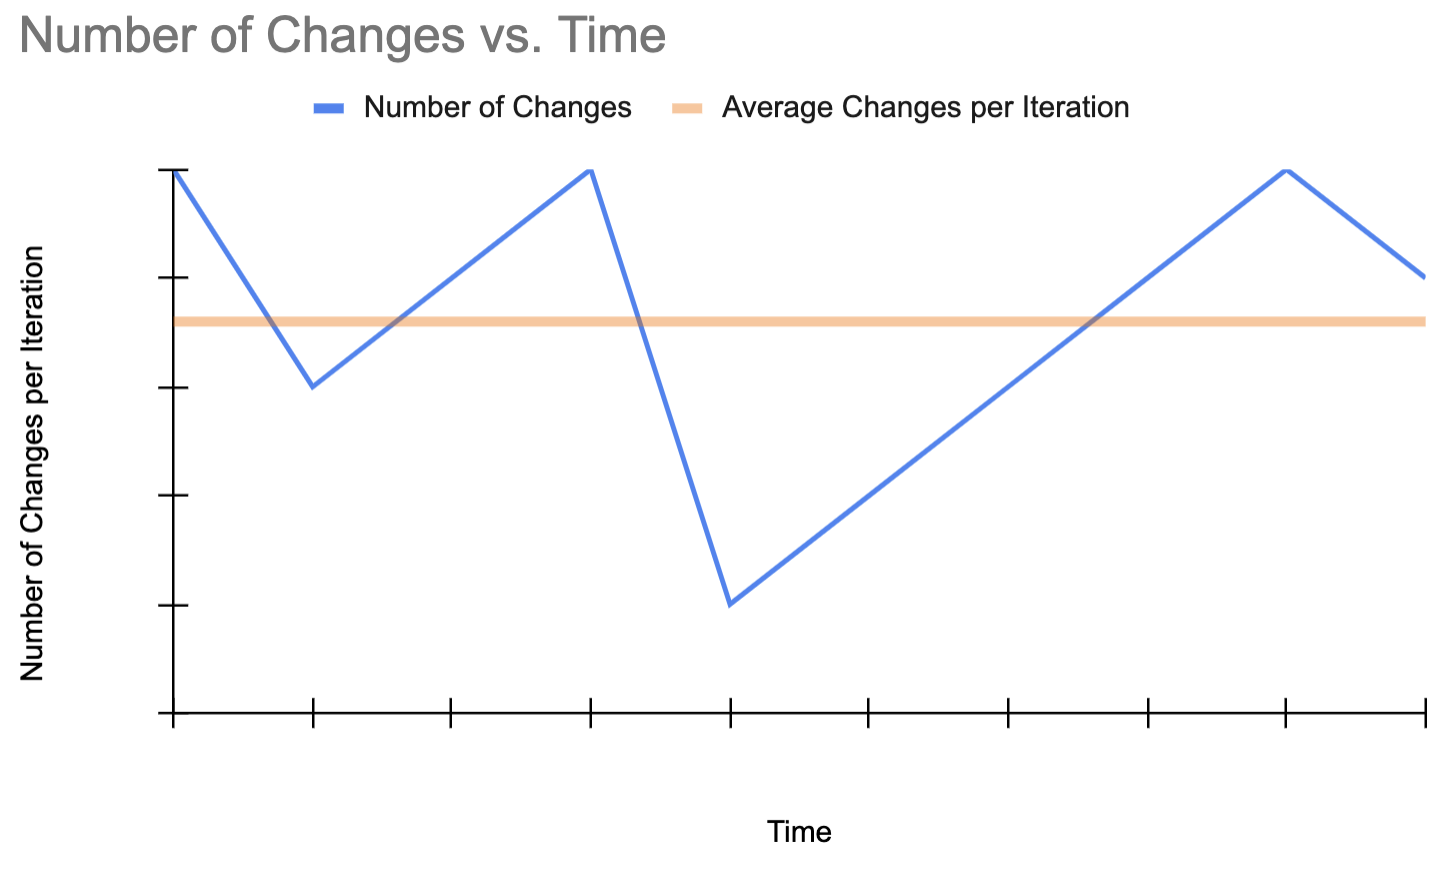
\includegraphics[width=\columnwidth]{Changes-vs-Time}
    }
    \caption{A simplified visual of Lehman's fifth law, ``Conservation of Familiarity.''}
    \label{figConservationOfFamiliarity}
\end{figure}

In Lehman's sixth law, ``Continuing Growth,'' we see that the system user's satisfaction will drop without continually increasing the functional content. Along with a similar idea, the law about ``Declining Quality'' states that if the operational environment for the system does not change, the system's quality will appear to decline. Yu and Mishra performed focused research on supporting Lehman's Laws, especially in the case of the seventh law about declining quality. They did this by defining a metric for software quality and reviewing the bug history, growth of the size, complexity, and quality of two large open-source systems \cite{yu:2013}. Therefore, we must continue adapting for even the appearance of the maintained quality of a system.

With many characteristics surrounding software evolution, we benefit from the Internet, which has positively improved the experience. Two common resources currently available to developers have impacted software evolution \cite{wiki:software-evolution}:

\vspace{0.25cm}
\begin{enumerate}
    \item The rapid growth of the World Wide Web and Internet Resources make it easier for users and engineers to find related information.
    \item Open source development where anybody could download the source codes and modify it has enabled fast and parallel evolution (through forks).
\end{enumerate}
\vspace{0.25cm}

These two suggestions are very evident in modern development. In other words, a developer may regularly use resources like StackOverflow to find solutions to problems and use open-source tools that the developer and their team can contribute to or adjust to their specific needs.

\subsection{Measuring Maintainability} \label{subMeasureMaintainability}

Despite the nuanced differences between \textit{maintainability} and \textit{evolution}, the two characteristics run parallel to each other. It will be easier to evolve if a system is easy to maintain. If we can measure our system's maintainability, we can also determine if our system is in a good position to continue evolving to meet our future needs.

\vspace{0.25cm}
\begin{displayquote}
``The unit cost of change must initially be made as low as possible and its growth, as the system ages, minimized. Programs must be made more alterable, and the alterability maintained throughout their lifetime. The change process itself must be planned and controlled.'' \cite{lehman:1980}
\end{displayquote}
\vspace{0.25cm}

Several tools attempt to provide some value around these ideas. In this paper, we will focus on the metrics that Pylint and Radon provide, specifically looking into their Refactor score of Pylint and the Maintainability Index from Radon.

We will look at many open-source Python systems using Radon and Pylint, then attempt to correlate the data from the scores to the level of ease in adding new features to the system.

% -----------------------------------------------------------------------------
% -  (B) We can use maintainability scores to see how structure impacts evolution.
% -----------------------------------------------------------------------------
\subsection{Maintainability Scores} \label{subMaintainabilityScores}

% --- Claim B: Review each claim from the introduction

First, let us consider our original interpretation of software maintainability. While this definition focuses primarily on bug fixes and minor enhancements, maintainable projects should also have ease in their ability to evolve. Therefore, we can study the impact maintainability (structural quality) has on software evolution by reviewing the scores provided by automated code review tools.

In this study, we will be using Pylint and will focus on the values of the Refactor score regarding a set of open-source Python systems. We must recognize what Pylint itself is doing to understand the scores we will be working with.

Through the documentation of Pylint, we can decipher how to use it and the scores it will provide \cite{pylint:main}. The Pylint score itself is calculated by the following equation \cite{pylint:score}:

\vspace{0.25cm}
\begin{center}
\code{10.0 - (( float( 5 * e + w + r + c) / s ) * 10 )}
\end{center}
\vspace{0.25cm}

Numbers closer to \code{10} reflect systems that have fewer errors, fewer warnings, and overall better structure and consistency. In the above equation, we are using the following values \cite{pylint:docs}:
\begin{singlespace}
  \begin{itemize}
    \item \textbf{statement} (\code{s}): the total number of statements analyzed
    \item \textbf{error} (\code{e}): the total number of errors, which are likely bugs in the code
    \item \textbf{warning} (\code{w}): the total number of warnings, which are python specific problems
    \item \textbf{refactor} (\code{r}): the total number of refactor warnings for bad code smells
    \item \textbf{convention} (\code{c}): the total number of convention warnings for programming standard violations
  \end{itemize}
\end{singlespace}

The Refactor score is of particular interest to us and considers many features meticulously outlined on the Pylint site \cite{pylint:refactor}. These types of warnings include many checks, like prompting when to simplify a boolean condition, a useless \code{return}, and more. This score, in particular, will be part of our focus.

Pylint will check the code for code smells based on the definitions for documented checks to calculate the Refactor score. For every infraction, the score increases by one count. 

% -- How Pylint Refactor errors are related to architecture smells ------------

\vspace{0.25cm}
\begin{displayquote}
  ``In computer programming, a \textbf{code smell} is any characteristic in the source code of a program that possibly indicates a deeper problem.'' \cite{wiki:code-smells}
\end{displayquote}
\vspace{0.25cm}

We can use these Refactor scores to help us spot architecture smells. After all, code smells can point the way to deeper problems in our system. However, there are fundamental established design principles that we should consider when creating software; code smells alert us to areas that have deviated from these principles. These smells are drivers for refactoring and when addressed, can help us maintain the integrity of our architecture rather than creating a patchwork construction. Because of the relation of refactoring scores to the code structure itself, we will be spending much of our focus on this particular value.

Furthermore, concerning Python, it is also helpful to be familiar with PEP 8, as this is the default set of standards that Pylint uses to judge Python code \cite{pylint:pep8}. This standard leads to making code more readable and more consistent, which may contribute to the code being more maintainable than without the standards. These standards cover things like indentation spacing, maximum line length, where to insert new lines, how to handle imports, and more. By defining a set of standards, teams can ensure they have a defined set of rules so that any contributors to the code understand the expectations (and so that automated systems like Pylint can enforce those standards to maintain readability and consistency).

Using Radon, we will also collect the Maintainability Index score. As mentioned earlier, many IDEs and other tools compute this value using a similar formula. Radon calculates the value using the following equation \cite{radon:docs}:

$$
MI = max[0, 100\frac{171 - 5.2 \ln{V} - 0.23G - 16.2 \ln{L} + 50 \sin{\sqrt{2.4C}}}{171}]
$$

\noindent
In this equation, we have the following values:
\begin{singlespace}
  \begin{itemize}
    \item $V$ is the Halstead Volume
    \item $G$ is the total Cyclomatic Complexity
    \item $L$ is the number of Source Lines of Code (SLOC)
    \item $C$ is the percent of comment lines (important: converted to radians)
  \end{itemize}    
\end{singlespace}

The Radon documents bring up the important note that the Maintainability Index is an experimental metric and should not be taken as seriously as other metrics. While it may be true that Maintainability Index is considered ``experimental,'' we will use this value as a primary indicator to look for correlations in the raw values we will collect.

% --- Claim B: Identify the evidence (analysis and comparison, theorems, measurements, case studies)

\subsection{Other Maintainability Characteristics} \label{subOtherCharacteristics}

The authors of ``Measurement and refactoring for package structure based on complex network'' recently reviewed a similar idea focusing on cohesion and coupling over time for a project \cite{zhou:2020}. In a software system, we desire low coupling (allowing for changes to one area to remain independent of changes to another area) and high cohesion (indicating reduced complexity in modules, which improves maintainability). Through a few experiments on open-source software systems, the authors determined that their algorithm that calculated metrics could improve package structures to have high cohesion and low coupling. Their study gives us confidence that metrics around the software's structure can provide value in keeping systems in a maintainable state, which allows for software evolution.

Another variable that may impact the maintainability of code is readability. For example, in the article ``How does code readability change during software evolution?'' the authors have addressed this concern and found that most source codes were readable within the sample they reviewed. Additionally, a minority of commits changed the readability; if a file is less readable, it was likely that it remained that way and did not improve \cite{piantadosi:2020}. This variable (readability) in the maintainability of a software system can influence how easy or difficult it is to make a change. The authors also found that big commits, usually associated with adaptive changes (a form of software evolution), were the most prone to reduce code readability \cite{piantadosi:2020}. We assume that smaller commits are almost always better and can lead to more readable code.

Piantadosi et al. found that changes in readability, whether improvements or disintegrations, often occurred unintentionally \cite{piantadosi:2020}. By enforcing the PEP 8 standard, we know that Pylint is encouraging systems to remain readable. Therefore, projects that use some form of automated system in their pipeline benefit from keeping their project on track, limiting the effects of readability on a software's potential for evolution.

The paper ``Standardized code quality benchmarking for improving software maintainability'' provides insights into how the code's maintainability is impacted by the technical quality of source code \cite{baggen:2012}. Within their paper, the authors seek to show four key points: (1) how easy it is to determine where and how the change is made, (2) how easy it is to implement the change, (3) how easy it is to avoid unexpected effects, and (4) how easy it is to validate the changes. Their approach has shown that some tools and methods can improve and maintain technical quality within their projects, allowing systems to continue to evolve at a reasonable pace.

% -----------------------------------------------------------------------------
% -  (C) Documentation can improve maintainability.
% -----------------------------------------------------------------------------
\subsection{Documentation and Maintainability} \label{subDocumentation}

% --- Claim C: Review each claim from the introduction

Our assumption is that the Refactor score in projects should correlate to the evolution of the system. The first pass through the data is not conclusive in this particular detail, as the projects reviewed have many other factors contributing to the evolution of the project (number of contributors, size of the code system, etc.). Our assumption is that the correlation between software quality and software evolution would indicate that the better-scoring code systems are readable in themselves. In addition, it would be helpful to understand whether there are any similarities in how a system is documented that could contribute to improved software evolution of a system.

% \todo{TODO: what kind of documentation do the ``good'' projects have?}

% \todo{TODO: what kind of documentation do the ``bad'' projects have?}

% --- Claim C: Identify the evidence (analysis and comparison, theorems, measurements, case studies)

The textbook, ``Software Architecture in Practice,'' chapter 18 provides some insight in documentation around architecture \cite{book:software-architecture-in-practice}:

\vspace{0.25cm}
\begin{displayquote}
  ``If you go to the trouble of creating a strong architecture, one that you expect to stand the test of time, then you \textit{must} go to the trouble of describing it in enough detail, without ambiguity, and organizing it so that others can quickly find and update the needed information.''
\end{displayquote}
\vspace{0.25cm}

The book describes how documentation holds the results of significant design decisions, providing valuable insights into decisions down the road. While not directly related to the Pylint Refactor score and not within the source code itself, it is still helpful to remind ourselves that documentation can also influence the ability of a software system to evolve.

\todo{Our ``best scores'' (regarding the current Pylint Refactor score) were found to have relatively organized and useful documentation. The code repository for \emph{Munki} provided documentation for previous versions, lending insight into design decisions as the software evolved \cite{data:munki}. The repository for \emph{Raven}, however, was a deprecated version that has since been replaced by a paid platform known as \emph{Sentry}, but had ample documentation \cite{data:raven-python}. It is possible that the ``death'' of that software system was not lack of evolution, but rather a business decision. \emph{ElastAlert} was another system with good scores and easy-to-follow documentation, though it is focused more for the use of the system rather than how to enhance the system itself \cite{data:elastalert}.}

\todo{When reviewing our ``worst offenders'' in current Refactor scores, it was noted that even with poor scores, these repositories were able to continue to see engagement from developers. While further inspection will be needed to understand whether the code itself is evolving or just has engagement from a maintenance level, it is interesting to note that there is decent documentation provided. \emph{SymPy} goes as far as documenting the architecture for the software as well as design decisions, enabling developers to better understand the structure as they make contributions \cite{data:sympy-docs}.}

\vspace{0.25cm}
\begin{displayquote}
  ``Our study has shown that the primary studies provide empirical evidence on the positive effect of documentation of designs pattern instances on programme comprehension, and therefore, maintainability.''
\end{displayquote}

\begin{displayquote}
  ``...developers should pay more effort to add such documentation, even if in the form of simple comments in the source code.''
\end{displayquote}
\vspace{0.25cm}

In research done by Wedyan and Abufakher (quoted above), it was found that documenting design patterns was useful in enhancing code understanding \cite{wedyan:2020}. In turn, the comprehensibility impacts the maintainability of the code in a positive way, which continues to reinforce the impact that documentation can have and how it ties well into considerations for software structure.

Borrego et al. discussed that software development teams must have access to architecture knowledge, as that is the base in which they will build and understand the technical part of any software development cycle \cite{borrego:2017}. It has also been recognized that an absence of knowledge management is a factor in failure of a development project \cite{borrego:2017}. 
Bjørnson and Dingsøyr noted that knowledge, in software engineering, is managed mostly through repositories that will support knowledge flows \cite{bjornson:2008}.

% =============================================================================
% =  Related Works
% =============================================================================

\section{Related Work} \label{sectionRelatedWork}

In our research, we are running with the assumption that Maintainability Index (MI) is our primary indicator. Therefore, we will look for the correlation between the MI and other Pylint scores.

\subsection{Considering Data Sets}

When exploring the correlations between maintainability and refactoring, many sources are available for research. For example, some researchers have looked at proprietary systems as they evolve, while others have chosen open-source code available to the general public.

A study conducted by Baishakhi Ray, Daryl Posnett, Premkumar Devanbu, and Vladimir Filkov begins by programmatically collecting a sample set of projects on GitHub that vary in languages. Then the group of projects is appropriately thinned out, resulting in a final set used for the review. The results are then studied for the impact different programming languages may have on the code quality \cite{baishakhi:2017}. Finally, their research determined which languages were more prone to defects and which individual languages were more related to individual bugs rather than bugs overall.

The authors of ``Predicting Maintainability with Object-Oriented Metrics - An Empirical Comparison'' performed a similar study to what we are doing here. Their study focuses on object-oriented software (specifically C/C++ and Java) and correlation analysis between object-oriented metrics and software maintainability. Janke et al. looked for the best metrics to predict maintainability \cite{janke:2003}. That study focused on a few hand-picked software systems with an analysis of the changelogs. Our study, in contrast, will be of a larger scale (about 50 software systems) and focused solely on Python-heavy projects.

\subsection{Design Patterns \& Software Quality}

In the paper ``Impact of design patterns on software quality: a systematic literature review'' the authors compared the use of design patterns to software evolution and maintainability. They found that design patterns provided flexibility when reviewing changes that extended (evolved) software \cite{wedyan:2020}.

\vspace{0.25cm}
\begin{displayquote}
  ``Changes performed in a class can be corrective, adaptive, perfective, or preventive. These changes can occur due to new requirements, debugging, changes that propagate from changes in other classes and refactoring.''
\end{displayquote}
\vspace{0.25cm}

Wedyan and Abufakher found that there were two reasons that a class had more frequent changes \cite{wedyan:2020}:

\vspace{0.25cm}
\begin{enumerate}
    \item The class was easy to extend.
    \item The class correlated to other classes (raising alarms about class modularity).
\end{enumerate}
\vspace{0.25cm}

With these findings in mind, we intentionally aim to focus our research on changes for system extensions and adaptations rather than bug fixes that appeared to be more considerable change due to high coupling. This paper focuses on Refactor scores (code smells) rather than Error scores (bugs) within the system.

\subsection{Software Architecture \& Maintainability}

In the research done in ``Software Architecture Metrics: A Literature Review'', the authors discuss how early detection of issues within the software's architecture is key to mitigating the risk of poor performance and can lower the cost of repairing faults \cite{coulin:2019}. While most developers have had access to these metrics for several decades, the industry and open-source community have not commonly adopted their use for keeping code in easy-to-work-with conditions.

The review done by Coulin et al. called out five essential qualities of software architecture \cite{coulin:2019}:

\vspace{0.25cm}
\begin{enumerate}
    \item Maintainability
    \item Extensibility
    \item Simplicity, Understandability
    \item Re-usability
    \item Performance
\end{enumerate}
\vspace{0.25cm}

Focusing on these qualities can narrow down the choice between different design options to an ideal solution. Keeping these five qualities in top-of-mind for new (and changed) code allows for easier future development and evolution of the software system.

ISO/IEC 25010:2011 is a detailed standard for software quality that contains eight product quality characteristics  \cite{iso/iec:25010:2011}. Each characteristic is further comprised of various sub-characteristics. ``Fig.~\ref{figProductQualityModel}'' lists these characteristics, with maintainability being one of the most significant characteristics in some studies \cite{gupta:2021}, \cite{adewumi:2016}.

\begin{figure}[ht]
  \centerline{
    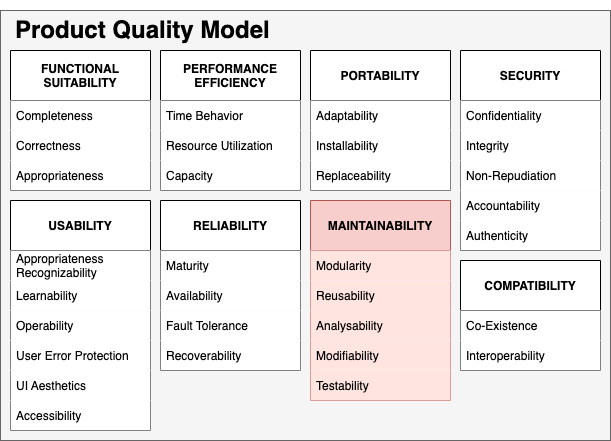
\includegraphics[width=0.7\columnwidth]{ProductQualityModel.png}
  }
  \caption{The eight product quality characteristics and sub-characteristics.}
  \label{figProductQualityModel}
\end{figure}


% Chapter three is how you did it.
\newpage
\chapter{Methodology} \label{chapterMethodology}

% In addition to the detailed methods you need to describe in this section, you need to provide specific objectives and an overview of your approach if they have not already been presented in the introductory chapters.  The best place to put those items can vary among theses.  Sometimes the background and lit review is really necessary to justify and substantiate the specific objectives and approach and, therefore, it is best to save those details for the beginning of this chapter.

There are a number of factors to consider when reviewing data and considering which software systems to consider. An obvious starting place is with open source software (OSS), as it is freely available to study.

To find projects of a caliber worth studying, we may also consider the maintenance capacity of a project.

\vspace{0.25cm}
\begin{displayquote}
  ``Maintenance capacity refers to the number of contributors to an OSS project and the amount of time they are willing and able to contribute to the development effort as observed from versioning logs, mailing lists, discussion forums and bug report systems. Furthermore, sustainability refers to the ability of the community to grow in terms of new contributors and to regenerate by attracting and engaging new members to take the place of those leaving the community.'' \cite{adewumi:2016}
\end{displayquote}
\vspace{0.25cm}

\section{Initial Repository Set} \label{sectionInitialSet}

We have established that we have a problem with projects that fail to evolve, resulting in a loss of revenue. We also understand that evolving software is essential in order to keep users engaged; without it, there is an appearance in the decline of quality and the program becomes less satisfactory to the user, as well as potential for competitors to outpace us with features available. We must now understand how we can ensure that our systems evolve. For this, we will look to understand how the system's structural quality impacts software evolution.

The work done by Dr. Omari and Dr. Martinez involves collecting a sub-set of Python projects that we can use for further research. The bulk of the effort they have provided is determining which classifiers to use to pare down the public set of Python systems into a good collection for further analysis \cite{omari:2018}. The work that they have provided was used to select appropriate Python systems for review by collecting meta-data on these code systems.

Selection criteria employed by Omari and Martinez included ``popular projects with long development history and multiple release cycles \cite{omari:2018}.'' All projects are open source, enabling other researchers to have access to the defined set. Additionally, they captured meta-data that was then used to define our own subset of repositories for our particular focus.

From their subset of repositories, we reviewed current Pylint scores from each of the 132 systems. This gives us a sampling of data that we can now dig deeper into, comparing similar systems (similar size, similar number of contributors, etc.) and their evolution process by reviewing past commits rather than merely the current state of the system, as we have done here.

\section{Filtered Respository Set} \label{sectionFilteredSet}

Once we had a narrowed set of projects from GitHub to ones primarily written in Python, we culled the set more using several criteria:

\vspace{0.25cm}
\begin{enumerate}
    \item Projects that are at least 80\% Python
    \item Projects with a long history of commits
    \item Projects with large development teams (community of contributors)
    \item Projects with many releases
    \item Projects of a substantial age
\end{enumerate}
\vspace{0.25cm}

Armed with this list, we were able to use the metadata from GitHub for each of our repositories already collected and determine a cross-section of these criteria that would result in about 50 repositories for further study.

Beginning with the languages field from GitHub, we could quickly narrow down projects that had at least 80\% of the code in Python. In our set, 103 repositories contained 80\% or more Python code.

With this narrowed set, we then looked to see which percentile all the remaining criteria would yield the desired number of repositories. We determined that using the value at the 20th percentile in each of the above categories would yield the size set we would need.

\begin{table}[ht]
  \centering
  \begin{tabularx}{0.8\textwidth} {
    | >{\centering\arraybackslash}X 
    | >{\centering\arraybackslash}X |
  }
    \hline
      Criteria & 20th Percentile Value \\ 
    \hline\hline
      Number of Commits & 2,968 \\
      Number of Contributors & 90 \\
      Number of Releases & 44 \\
      Age (in months) & 66.4 \\
    \hline
  \end{tabularx}
  \caption{Criteria used to filter down the initial set of repositories.}
  \label{table:repositoryPercentiles}
\end{table}

Table \ref{table:repositoryPercentiles} shows the values found for each of our criteria. Using these values as our minimum requirements, we can narrow our repository set to 46 repositories (see Table \ref{table:repositorySet}).

\begin{table}[ht]
  \centering
  \begin{tabularx}{1.0\textwidth} {
    | >{\centering\arraybackslash}X |
  }
    \hline
      Respository Names \\ 
    \hline\hline
      ansible
      astropy
      autobahn-python
      aws-cli
      beets
      biopython
      boto
      buildbot
      celery
      cobbler
      conda
      cython
      django
      django-rest-framework
      electrum
      fail2ban
      gensim
      luigi
      matplotlib
      mongoengine
      mitmproxy
      mongo-python-driver
      mopidy
      networkx
      paramiko
      nova
      numba
      pandas
      peewee
      pelican
      pip
      pyramid
      ranger
      raven-python
      salt
      scikit-image
      scikit-learn
      scrapy
      sentry
      sqlalchemy
      swift
      sympy
      tornado
      web2py
      werkzeug
      youtube-dl \\
    \hline
  \end{tabularx}
  \caption{List of the 46 repositories for research focus.}
  \label{table:repositorySet}
\end{table}


% Chapter four is what you found.
\newpage
\chapter{Results} \label{chapterResults}

% Results, findings, discussion of results OR manuscripts. It is best to reiterate information in your literature review to help substantiate your research findings.

With our narrowed focus on repositories, we can now spend more time looking through the data collected. Specifically, we gathered data on the Refactor Warnings provided by Pylint. In Table \ref{table:smallRefactorWarningTotals} we have a shortened listing of the repositories from our set with their total count of refactoring warning messages, in addition to the most commonly appearing to refactor warning message. For the entire set, see Table \ref{table:allRefactorWarningTotals} in the Appendix.

\begin{table}[ht]
  \small
  \centering
  \begin{tabularx}{0.8\textwidth} {
    | l 
    | c
    | >{\centering\arraybackslash}X 
    | c |
  }
    \hline
    Repository Name & Msg Count & Top Msg & Top Msg Count \\
    \hline\hline
    sympy & 14,206 & too-many-arguments & 6,601 (46\%) \\ \hline
    ansible &  10,431 & no-else-return & 1,711 (16\%) \\ \hline
    salt &  7,814 & too-many-arguments & 1,640 (21\%) \\ \hline \hline
    ranger & 109 & no-else-return & 29 (27\%) \\ \hline
    sentry & 66 & no-self-use & 32 (48\%) \\ \hline
    raven-python & 20 & too-few-public-methods & 7 (35\%) \\ \hline
  \end{tabularx}
  \caption{Total refactor messages per repository for the 3 best and 3 worst offendors. Also provided with the refactor message that had the most warnings and its total count (and the percentage of that message from the total refactor warnings for that repository).}
  \label{table:smallRefactorWarningTotals}
\end{table}

Regarding the number of refactoring warning messages, we can see that the ``worst'' project in our set was the repository Sympy \cite{data:sympy}, with 14,206 refactor messages. However, project size may also weigh how many warnings and errors are present, as projects with more lines of code are presumed to have more errors.

If we instead look at the ratio of refactoring warnings to the total lines of source code, we get a very different picture, provided in Table \ref{table:smallRefactorSLOCRatio}. We calculated these values using the following equation, $r$ is the total refactor message count for the project, $c$ is the total number of source lines of code in the project, and 100 is a multiplier to make the numbers easier to wrap our heads around. So the numbers closer to 0 are better ratios, as there are fewer refactor messages in the project relative to its size.

$$
Refactor \space Ratio = r / c * 100
$$

In this case, the repository Raven-Python \cite{data:raven-python} (which was the ``best'' in regards to total refactor message count) is now the ``worst'' with the highest ratio of refactoring warnings compared to the lines of source code in the project. Raven-Python also has the least count of SLOC in the entire repository set!

\begin{table}[ht]
  \small
  \centering
  \begin{tabularx}{1.0\textwidth} {
    | l 
    | r
    | r
    | >{\centering\arraybackslash}X |
  }
    \hline
    Repository & Total Refactor Msgs & Total Project SLOC & Ratio \\
    \hline\hline
    raven-python & 20 & 1,474 & 1.35 \\ \hline
    scrapy & 381 & 58,768 & 0.64 \\ \hline
    numba & 126 & 20,192 & 0.62 \\ \hline \hline
    electrum & 722 & 425,576 & 0.16 \\ \hline
    youtube-dl & 1,003 & 667,075 & 0.15 \\ \hline
    cython & 1,718 & 1,183,863 & 0.14 \\ \hline
  \end{tabularx}
  \caption{Total refactor messages per repository, total project source line of code (SLOC), and the ratio of refactor messages to SLOC.}
  \label{table:smallRefactorSLOCRatio}
\end{table}

Given that we now have an idea of which projects have the most refactor messages per line of source code (``worst'' offenders) and the projects with the least refactor messages (``best'' projects for maintainability), we can look a little closer at the most frequent messages. For example, common to all six repositories at a high frequency is the message ``no-self-use'' and ``no-else-return''. The message ``no-self-use'' means that `self' is used as an argument but not in the method; this should be handled differently. For example, the message ``no-else-return'' highlights when an unnecessary code block follows an if-conditional.

Some of the other common messages call out the use of ``too many'' of different types of objects. For example, ``too-many-branches'', ``too-many-arguments'', ``too-many-locals'', ``too-many-statements''... 

\vspace{0.25cm}
\begin{displayquote}
  ``Software maintainability these days has become one of the essential external attributes of software, which further forms a basis of research for many researchers working in the fields related to software engineering. Software maintainability can be described as how a particular software system can be changed concerning the number of Lines of Code (LOC).'' \cite{gupta:2021}
\end{displayquote}
\vspace{0.25cm}

Now, it would be helpful to understand where we stand on the Maintainability Index (MI) for these projects, as this is our form of measurement that will help us understand how the code might be able to evolve. The MI is calculated on a per-module basis, but for the sake of conversation (and acknowledging that we will lose some nuances by reducing it this way), let us find the average MI at the project level and add this to our table (Table \ref{table:smallRefactorSLOCRatio2}). Also included is the standard deviation for each average, with the lowest standard deviation being 13.75 and the highest at 31.14. Most averages have a standard deviation between 20 and 30 points.

\begin{table}[ht]
  \small
  \centering
  \begin{tabularx}{1.0\textwidth} {
    | l 
    | r
    | r
    | r
    | >{\centering\arraybackslash}X |
  }
    \hline
    Repo & Refactor Msgs & Project SLOC & Ratio & Avg Project MI \\
    \hline\hline
    raven-python & 20 & 1474 & 1.35 & 87.02 ±13.75 \\ \hline
    scrapy & 381 & 58768 & 0.64 & 64.47 ±17.72 \\ \hline
    numba & 126 & 20192 & 0.62 & 62.55 ±21.08 \\ \hline \hline
    electrum & 722 & 425576 & 0.16 & 39.41 ±28.06 \\ \hline
    youtube-dl & 1003 & 667075 & 0.15 & 54.16 ±19.95 \\ \hline
    cython & 1718 & 1183863 & 0.14 & 31.02 ±29.19 \\ \hline
  \end{tabularx}
  \caption{Total refactor messages per repository, total project source line of code (SLOC), the ratio of refactor messages to SLOC, average Maintainability Index (MI).}
  \label{table:smallRefactorSLOCRatio2}
\end{table}

\todo{With our more minor data set on hand, we ran Radon against each repository to gain a Maintainability Index. We averaged the Maintainability Index of all files within each project for a very simplified view. This gave us a single number for general comparison with each repository.}

\todo{The ``Avg MI'' column in the table contains the calculated average value for each file in the project. In Radon's grading system, any value over 20 is considered a ``very maintainable'' code. We also used a count of the Pylint REFACTOR messages and calculated the ratio of messages to source-line-of-code for how many code smells each project contained relative to its size. This calculated ratio is shown in the ``Ratio'' column. Listed in the table are the ``best 3'' (cython, youtube-dl, and electrum) and the ``worst 3'' (raven-python, scrapy, and numba) regarding their refactor ratios.}

When reviewing the Maintainability Inde for our repositories at either end of the spectrum and in context with the entire set (see Appendix \ref{table:allRefactorSLOCRatio}), we will find that while Raven-Python has the highest number of refactoring warnings when compared to the SLOC count. Raven-Python also has the second-highest average MI across all of its project files.

Of the entire set, our highest average MI is 87.38 ±19.47 (belonging to Sentry), and our lowest average MI is 28.85 ±27.37 (belonging to MatPlotLib). Regardless, these average values are above a score of 20, which is Radon's lowest score provided for an ``A'' rank, that is, what would be considered a project ``very high'' maintainability.

With this information, we can get an idea of where these projects stand regarding their refactor message ratios compared to each other. For example, the histogram in Fig. \ref{figHistogramRefactorRatio} shows that the majority of our repository set has a meager ratio of refactoring messages. However, the mass projects on the low-end could indicate that our projects are highly maintainable based on our assumptions that refactor messages are related to maintainability. Having few refactor messages (relative to the number of lines of code) means we have a smaller number of code smells. Therefore, infrequent refactor warnings are helpful for our architecture and quality!

\begin{figure}[ht]
  \centerline{
    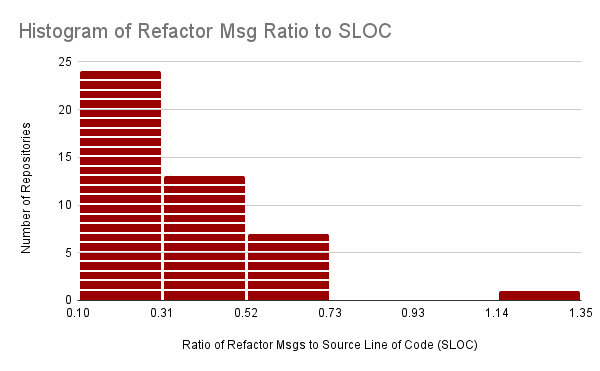
\includegraphics[width=0.8\columnwidth]{Histogram of Refactor Msg Ratio to SLOC.png}
  }
  \caption{Histogram of the number of refactor messages relative to the size of the project as measured by source lines of code. Diligent development communities can keep refactor warnings low, regardless of system size (lines of code).}
  \label{figHistogramRefactorRatio}
\end{figure}

The data set we chose may impact the ratios, lending to them all being on the low end. Perhaps open-source projects with highly engaged communities tend to keep their code in a maintainable state because this would be the only way for significant involvement (over 90 contributors per project). It has been interesting to see how low the ratio of refactoring messages has been in our data set.

To view the same repository set with their Maintainability Index averages, we have another histogram in Fig. \ref{figHistogramAvgMI}. This Radon score can range from 0 (awful) to 100 (perfect). Radon considers any value above 20 to be an ``A'' or ``very maintainable''. All of our projects receive an ``A'' grade, with the majority in the middle range (around 40 to 50). All projects in our data set were all mid-to high-range scores.

\begin{figure}[ht]
  \centerline{
    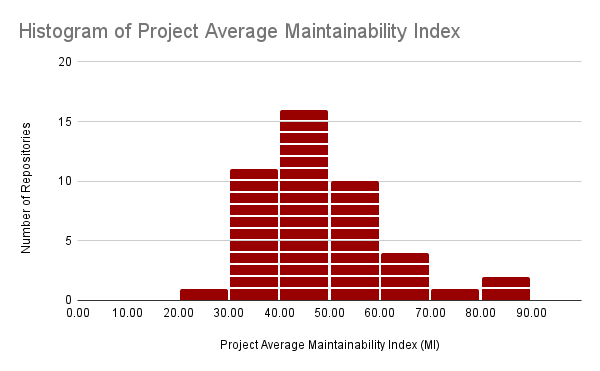
\includegraphics[width=0.8\columnwidth]{Histogram of Project Average Maintainability Index_BucketSize_10.png}
  }
  \caption{Historgram of project average Maintainability Index (MI).}
  \label{figHistogramAvgMI}
\end{figure}


% Chapter five is what it all means – putting the pieces together, (what’s your contribution to the research field).
\newpage
\chapter{Conclusions and Recommendations} \label{chapterConclusion}

% This chapter could also be called "Conclusions and Recommendations" or "Conclusions and Implications." In general, there should be no new information presented here. Instead, it should be a synthesis of information that you have already discussed. 

By collecting data and drawing our conclusions from it, with help from the insights from the studies done before ours, we may better understand metrics that can be useful regarding maintainability. Good projects will inevitably continue to grow and evolve. For example, understanding methods to keep code refactor on a certain level makes code easy to change. We may also find that projects with worsening scores slow down with updates and have reduced engagement.

When reviewing our data with current project Refactor message ratios, our three worst offenders were \emph{Raven-Python}, \emph{Scrapy}, and \emph{Numba} \cite{data:raven-python}, \cite{data:scrapy}, \cite{data:numba}.  \emph{Raven-Python} has been deprecated in favor of a newer system,  \emph{Sentry-Python}. Despite their poor scores, the other two projects are still active in development. The two active projects are included in thousands of projects each, which may be the reason for continued development despite the potential difficulty in maintenance.

Projects that may be open source or have many contributors are especially vulnerable to maintainability degrading over the evolution of a project. Having a reliable metric can be very useful in programmatically avoiding code smells and keeping code in a state that is easy to manage through simple metric checks in deployment pipelines.

While not one of our worst refactor-to-SLOC ratios, \emph{SymPy} is a repository with a large number of refactoring warnings. We can see an example of code smell issues in reviewing some current symptoms that \emph{SymPy} is experiencing, with only 72\% code coverage and a failing build (see "Fig.~\ref{figSymPyStatus}"). Despite the engagement and continued development, we suspect that the actual adaptations and evolution of the software may be complex with this code.

\begin{figure}[ht]
  \centerline{
    
\includegraphics[width=1.0\columnwidth]{SymPy_status}
  }
  \caption{A snapshot of the badges from \emph{SymPy}'s repository.}
    \label{figSymPyStatus}
\end{figure}

\todo{We have further work to do in this study to gain a better understanding. With several "best" and "worst" Python software systems, we will look into the history of the projects' commits. It would be helpful to see how the Refactor scores have changed over time and if the rate at which changes were pushed correlated to the increase or decrease in that Refactor score.}

\todo{Additional data can be gathered from this set that may provide more insights than this first brush of the data provides us. Understanding the impact of structural quality on the evolution of a project can provide compelling perspectives.}

From our set, the very best and worst repositories are still actively improving and evolving, even today. An exception to this is our "worst" repository, raven-python, which was deprecated (this means the code is no longer supported), but in exchange for an improved system. The raven-python community did not die but instead recognized that a better architecture was needed for the system to continue to evolve. So they built a new code system (Sentry-Python) and shifted support there, where they have a better architecture and ability to evolve.

Open-source systems and any project with many contributors or have many changes are vulnerable to degrading quality. It is just the nature of change over time. However, when we review a set of popular repositories that already have a long history of commits (these repositories are still active and over five years old!), we find that they have good maintainability.

Where do we go from here? Regarding the data, we would like to do more studies to understand the correlation between the Pylint metrics and Maintainability Index to gain better insights into our assumptions.

So far, we have found a reinforcement of what many of us already know. Good architecture is vital for software to be able to evolve. Reliable quality metrics can help keep an architecture ready for enhancements. Regardless of the codebase, teams should understand what standards will work best for their software solution. Then auto-enforce these standards in the development pipeline. Automated pipelines keep everyone honest and will improve the project's ability to evolve.


% =============================================================================
% =  References
% =============================================================================

\newpage
\begin{singlespace}
  \section*{References} \label{sectionReferences}

Includes all references: articles, media facts, books, reports, regulations, internet articles, papers that you referenced from the text.  In the text, citations can be (Smith and Jones, 2007) or Smith et al., 2007) (if more than two authors) if you wish to present your references alphabetically.  Alternatively, you can include the citations in the text as a number [1] or 1 if you wish to present your references numerically.  The MS WORD tools – “insert, reference, footnote, endnote” (or “cross reference” if you refer to the same reference more than once) should be used to help you organize and manage your references.

References can be written in single space with extra space between references as in the format below.  There are many different ways to arrange the information and punctuation in a reference listing.  The most important thing is to make sure all references are complete and that the format of your references is consistent throughout. 

Example, S.Z. (2008). How to cite a complete journal reference. J. Complete Thesis. 1(2): 47-52.

Example, S.Z., Second, W.S. (2007). How to cite a complete conference proceedings paper. In: Proceedings, 2nd International meeting of Masters Students, Paper \# XW15 (Potsdam NY, November, 2007).

If you use the “thesis” reference” style you will get the proper line spacing and indent style without further changes. Above are examples to show complete citation, other formats also acceptable.

\subsection*{Alternative format:}
An alternative format for references is to use IEEE format. You can find a reference on IEEE format here: http://www.ijssst.info/info/IEEE-Citation-StyleGuide.pdf

You can use either the option provided above in the template or use the IEE format. 

We should cite something \cite{omari:2018}.

% =============================================================================
% =  Bibliography and Sources
% =============================================================================

\newpage
\bibliographystyle{IEEEtran}
\bibliography{bibliography}

\end{singlespace}

% =============================================================================
% =  Appendices
% =============================================================================

\newpage
\setcounter{chapter}{7}

\chapter*{Appendix} \label{chapterAppendix}
\addcontentsline{toc}{chapter}{Appendix}

\section{Pylint: Refactor Scores} \label{appendixPylintRefactor}

The score in Pylint is a value out of 10, with 10 being the best. Pylint has a number of types of messages:
\begin{singlespace}
  \begin{enumerate}
    \item Convention
    \item Error
    \item Fatal
    \item Information
    \item Refactor
    \item Warning
  \end{enumerate}
\end{singlespace}

There is a very large list of all messages at \href{https://pylint.pycqa.org/en/latest/messages/messages_list.html}{Overview of All Pylint Messages}.

We spend most of our time reviewing the Refactor messages, found at \href{https://pylint.pycqa.org/en/latest/messages/messages_list.html#refactor}{Pylint Refactor Messages}.

Additionally, the Convention messages are also helpful for review, found at \href{https://pylint.pycqa.org/en/latest/messages/messages_list.html#convention}{Pylint Convention Messages}.

\section{Radon: Maintainability Index} \label{appendixRadonRefactor}

In this paper, we use Radon as one method for finding the Maintainability Index (MI) for projects, at the module (file) level. This grading scale is provided by Radon to align with its scores \cite{radon:docs}.

\begin{center}
  \begin{tabular}{ c c c }
    MI Score & Rank & Maintainability \\ \hline\hline
    100 - 20 & A & Very high \\ \hline
    19 - 10 & B & Medium \\ \hline
    9 - 0 & C & Extremely Low \\ \hline    
  \end{tabular}
\end{center}

\section{Data: Repository Refactor Messages} \label{appendixRefactorCounts}

\begin{singlespace}
  \begin{verbatim}
    -- Find total number of refactor messages
    SELECT 
      t1.name AS "Repository Name",
      SUM(t1.n::numeric) AS "Total Refactor"
    FROM pylint_metrics_by_msg AS t1
      WHERE t1.code = 'R'
    GROUP BY t1.name
    ORDER BY SUM(t1.n::numeric) DESC;

    -- Find "worst offender" messages for each repository
    SELECT
      t2.name AS "Repository Name",
      t2.msg AS "Most Common Refactor Message",
      SUM(t2.n::numeric) AS "Most Common Refactor Message Count"
    FROM pylint_metrics_by_msg AS t2
      WHERE name = 'sympy'  -- set repository name here
      AND code = 'R'
    GROUP BY t2.name, t2.msg
    ORDER BY SUM(t2.n::numeric) DESC
    LIMIT 1;
  \end{verbatim}
\end{singlespace}

\begin{table}[ht]
  \scriptsize
  \centering
  \begin{tabularx}{1.0\textwidth} {
    | l 
    | c
    | >{\centering\arraybackslash}X 
    | c |
  }
    \hline
    Repository Name & Msg Count & Top Msg & Top Msg Count \\
    \hline\hline
    sympy & 14,206 & too-many-arguments & 6,601 (46\%) \\ \hline
    ansible & 10,431 & no-else-return & 1,711 (16\%) \\ \hline
    salt & 7,814 & too-many-arguments & 1,640 (21\%) \\ \hline
    nova & 2,593 & no-self-use & 679 (26\%) \\ \hline
    sqlalchemy & 2,040 & no-else-return & 700 (34\%) \\ \hline
    astropy & 1,965 & no-else-return & 503 (26\%) \\ \hline
    biopython & 1,930 & no-else-return & 273 (14\%) \\ \hline
    matplotlib & 1,926 & too-many-arguments & 381 (20\%) \\ \hline
    django & 1,720 & no-else-return & 397 (23\%) \\ \hline
    cython & 1,718 & no-else-return & 417 (24\%) \\ \hline
    celery & 1,626 & no-self-use & 775 (48\%) \\ \hline
    web2py & 1,555 & no-else-return & 240 (15\%) \\ \hline
    scikit-learn & 1,485 & too-many-arguments & 363 (24\%) \\ \hline
    boto & 1,398 & too-many-arguments & 298 (21\%) \\ \hline
    pip & 1,215 & no-else-return & 191 (16\%) \\ \hline
    pandas & 1,197 & useless-object-inheritance & 316 (26\%) \\ \hline
    swift & 1,159 & too-many-arguments & 190 (16\%) \\ \hline
    buildbot & 1,129 & no-self-use & 177 (16\%) \\ \hline
    youtube-dl & 1,003 & too-many-locals & 413 (41\%) \\ \hline
    electrum & 722 & no-self-use & 163 (23\%) \\ \hline
    conda & 660 & no-else-return & 177 (27\%) \\ \hline
    aws-cli & 585 & no-self-use & 177 (30\%) \\ \hline
    networkx & 568 & too-many-locals & 124 (22\%) \\ \hline
    autobahn-python & 541 & useless-object-inheritance & 97 (18\%) \\ \hline
    scikit-image & 499 & too-many-arguments & 134 (27\%) \\ \hline
    mitmproxy & 488 & no-self-use & 133 (27\%) \\ \hline
    beets & 471 & no-else-return & 137 (29\%) \\ \hline
    pyramid & 452 & useless-object-inheritance & 116 (26\%) \\ \hline
    mongo-python-driver & 418 & too-many-arguments & 100 (24\%) \\ \hline
    scrapy & 381 & useless-object-inheritance & 102 (27\%) \\ \hline
    werkzeug & 348 & useless-object-inheritance & 95 (27\%) \\ \hline
    tornado & 326 & useless-object-inheritance & 71 (22\%) \\ \hline
    luigi & 299 & no-self-use & 77 (26\%) \\ \hline
    paramiko & 257 & no-self-use & 60 (23\%) \\ \hline
    django-rest-framework & 241 & no-self-use & 65 (27\%) \\ \hline
    cobbler & 221 & no-self-use & 64 (29\%) \\ \hline
    mopidy & 211 & no-self-use & 54 (26\%) \\ \hline
    peewee & 163 & useless-object-inheritance & 30 (18\%) \\ \hline
    fail2ban & 157 & no-else-return & 30 (19\%) \\ \hline
    mongoengine & 145 & no-else-return & 21 (14\%) \\ \hline
    numba & 126 & too-few-public-methods & 54 (43\%) \\ \hline
    pelican & 117 & no-else-return & 18 (15\%) \\ \hline
    ranger & 109 & no-else-return & 29 (27\%) \\ \hline
    sentry & 66 & no-self-use & 32 (48\%) \\ \hline
    raven-python & 20 & too-few-public-methods & 7 (35\%) \\ \hline
  \end{tabularx}
  \caption{Total refactor messages per repository. Also provided with the refactor message that had the most warnings and its total count (and the percentage of that message from the total refactor warnings for that repository).}
  \label{table:allRefactorWarningTotals}
\end{table}

\section{Data: Repository Refactor-to-SLOC Ratio} \label{appendixRefactorRatio}

It is good to note that the value for the Source Line of Code (SLOC), when added to multi-line comments, single-line comments, and blank lines, should add up to the total lines of code in the project \cite{radon:docs}. For this table, we are looking only at the SLOC, which are lines that are only actual code (no comments or blank lines).

\begin{singlespace}
  \begin{verbatim}
    SELECT
      t1_radon_raw.name AS "Repository",
        SUM(
          CASE
            WHEN t3_python_metrics.code = 'R' THEN n::numeric
            ELSE 0
          END
        ) AS "Total Refactor Msgs",
      SUM(t1_radon_raw.sloc::numeric) AS "Total Project SLOC",
      CONCAT(TRUNC(
          SUM(
            CASE
              WHEN t3_python_metrics.code = 'R' THEN n::numeric
              ELSE 0
            END
          ) / SUM(t1_radon_raw.sloc::numeric) * 100,
          2 -- Number of decimal places
        ), '') AS "Ratio",
        TRUNC(AVG(t2_radon_mi.mi::numeric), 2) AS "Average Project MI",
        CASE
          WHEN AVG(t2_radon_mi.mi::numeric) >= 20 THEN 'A'
          WHEN AVG(t2_radon_mi.mi::numeric) >= 10 THEN 'B'
          ELSE 'C'
        END AS "MI Rank",
        CASE
          WHEN AVG(t2_radon_mi.mi::numeric) >= 20 THEN 'Very high'
          WHEN AVG(t2_radon_mi.mi::numeric) >= 10 THEN 'Medium'
          ELSE 'Extremely low'
        END AS "Maintainability",
        CONCAT(TRUNC(
          SUM(t1_radon_raw.comments::numeric) 
            / SUM(t1_radon_raw.sloc::numeric) 
            * 100, 
          2  -- Number of decimal places
        ), '%') AS "Total Project Comment-to-SLOC Ratio"
    FROM new_radon_raw_metrics AS t1_radon_raw
    INNER JOIN new_radon_mi_metric AS t2_radon_mi
      ON t1_radon_raw.module_name = t2_radon_mi.module_name
        INNER JOIN new_pylint_metrics_by_msg AS t3_python_metrics
          ON t1_radon_raw.module_name = t3_python_metrics.module_name
            INNER JOIN new_repo_details AS t4_repo_details
              ON t1_radon_raw.name = t4_repo_details.repo_name_2
    GROUP BY t1_radon_raw.name
    ORDER BY (
      SUM(
          CASE
          WHEN t3_python_metrics.code = 'R' THEN n::numeric
          ELSE 0
          END
        ) / SUM(t1_radon_raw.sloc::numeric)
    ) DESC;    
  \end{verbatim}
\end{singlespace}

\newpage
\begin{table}[ht]
  \tiny
  \centering
  \begin{tabularx}{1.2\textwidth} {
    | l 
    | r
    | r
    | r
    | r
    | r
    | r
    | >{\centering\arraybackslash}X |
  }
    \hline
    Repository & Refactor Msgs & Project SLOC & Ratio & Avg Project MI & MI Rank & Maintainability & Comment-to-SLOC Ratio \\ \hline\hline
    raven-python & 20 & 1474 & 1.35 & 87.02 & A & Very high & 8.41\% \\ \hline
    scrapy & 381 & 58768 & 0.64 & 64.47 & A & Very high & 5.59\% \\ \hline
    numba & 126 & 20192 & 0.62 & 62.55 & A & Very high & 13.11\% \\ \hline
    sentry & 66 & 10770 & 0.61 & 87.38 & A & Very high & 8.89\% \\ \hline
    boto & 1398 & 237761 & 0.58 & 58.00 & A & Very high & 14.91\% \\ \hline
    celery & 1626 & 302080 & 0.53 & 41.73 & A & Very high & 6.00\% \\ \hline
    pyramid & 452 & 85302 & 0.52 & 70.25 & A & Very high & 10.29\% \\ \hline
    mopidy & 211 & 40381 & 0.52 & 59.15 & A & Very high & 7.19\% \\ \hline
    sympy & 14206 & 2873930 & 0.49 & 31.16 & A & Very high & 8.08\% \\ \hline
    aws-cli & 585 & 126303 & 0.46 & 61.73 & A & Very high & 15.89\% \\ \hline
    luigi & 299 & 68973 & 0.43 & 53.56 & A & Very high & 14.81\% \\ \hline
    networkx & 568 & 147166 & 0.38 & 44.66 & A & Very high & 24.00\% \\ \hline
    scikit-learn & 1485 & 396109 & 0.37 & 41.74 & A & Very high & 13.88\% \\ \hline
    peewee & 163 & 44595 & 0.36 & 31.26 & A & Very high & 4.76\% \\ \hline
    mongo-python-driver & 418 & 117448 & 0.35 & 43.62 & A & Very high & 12.44\% \\ \hline
    buildbot & 1129 & 318794 & 0.35 & 56.60 & A & Very high & 17.88\% \\ \hline
    django & 1720 & 485681 & 0.35 & 57.28 & A & Very high & 12.97\% \\ \hline
    pandas & 1197 & 357537 & 0.33 & 42.07 & A & Very high & 9.24\% \\ \hline
    mitmproxy & 488 & 148319 & 0.32 & 56.21 & A & Very high & 5.60\% \\ \hline
    biopython & 1930 & 615445 & 0.31 & 43.54 & A & Very high & 17.19\% \\ \hline
    django-rest-framework & 241 & 77488 & 0.31 & 50.68 & A & Very high & 9.35\% \\ \hline
    werkzeug & 348 & 116937 & 0.29 & 34.06 & A & Very high & 6.20\% \\ \hline
    autobahn-python & 541 & 182842 & 0.29 & 46.86 & A & Very high & 19.61\% \\ \hline
    sqlalchemy & 2040 & 703340 & 0.29 & 32.98 & A & Very high & 7.17\% \\ \hline
    cobbler & 221 & 77348 & 0.28 & 58.76 & A & Very high & 12.01\% \\ \hline
    scikit-image & 499 & 187819 & 0.26 & 53.87 & A & Very high & 9.64\% \\ \hline
    nova & 2593 & 981563 & 0.26 & 64.72 & A & Very high & 16.51\% \\ \hline
    paramiko & 257 & 97387 & 0.26 & 43.79 & A & Very high & 13.78\% \\ \hline
    tornado & 326 & 123535 & 0.26 & 37.14 & A & Very high & 17.28\% \\ \hline
    conda & 660 & 260363 & 0.25 & 44.82 & A & Very high & 16.42\% \\ \hline
    beets & 471 & 186165 & 0.25 & 43.66 & A & Very high & 15.64\% \\ \hline
    astropy & 1965 & 780617 & 0.25 & 40.20 & A & Very high & 19.38\% \\ \hline
    salt & 7814 & 3131332 & 0.24 & 45.69 & A & Very high & 8.43\% \\ \hline
    ranger & 109 & 44487 & 0.24 & 45.74 & A & Very high & 9.49\% \\ \hline
    pelican & 117 & 48096 & 0.24 & 35.95 & A & Very high & 7.82\% \\ \hline
    swift & 1159 & 523880 & 0.22 & 37.13 & A & Very high & 14.30\% \\ \hline
    pip & 1215 & 590140 & 0.20 & 47.52 & A & Very high & 12.61\% \\ \hline
    matplotlib & 1926 & 943406 & 0.20 & 28.85 & A & Very high & 11.10\% \\ \hline
    fail2ban & 157 & 84340 & 0.18 & 48.41 & A & Very high & 30.77\% \\ \hline
    mongoengine & 145 & 80473 & 0.18 & 30.75 & A & Very high & 9.24\% \\ \hline
    ansible & 10429 & 5818380 & 0.17 & 46.82 & A & Very high & 5.98\% \\ \hline
    web2py & 1555 & 903496 & 0.17 & 37.78 & A & Very high & 10.16\% \\ \hline
    electrum & 722 & 425576 & 0.16 & 39.41 & A & Very high & 9.14\% \\ \hline
    youtube-dl & 1003 & 667075 & 0.15 & 54.16 & A & Very high & 5.04\% \\ \hline
    cython & 1718 & 1183863 & 0.14 & 31.02 & A & Very high & 12.74\% \\ \hline
  \end{tabularx}
  \caption{Total refactor messages per repository, total project source line of code (SLOC), the ratio of refactor messages to SLOC, average Maintainability Index (MI), and code comment-to-SLOC ratio.}
  \label{table:allRefactorSLOCRatio}
\end{table}

\newpage
\section{Data: Repository Refactor By Message} \label{appendixRefactorMsgCounts}

This section contains information from the repositories that were on the edges of refactor message counts.

The sections for the projects with the highest ratio of refactor messages compared to the source lines of code are contained in Subsections \ref{appendixSubRavenPython} (Raven-Python), \ref{appendixSubScrapy} (Scrapy), and \ref{appendixSubNumba} (Numba).

The sections for the projects with the lowest ratio of refactor messages compared to the source lines of code are contained in Subsections \ref{appendixSubCython} (Cython), \ref{appendixSubYouTube} (YouTube-DL), and \ref{appendixSubElectrum} (Electrum).

The sections for the projects with the most total refactor messages are contained in Subsections \ref{appendixSubSympy} (Sympy),  \ref{appendixSubAnsible} (Ansible), and \ref{appendixSubSalt} (Salt).

\begin{singlespace}
  \begin{verbatim}
    SELECT
      t2.name AS "Repository Name",
      t2.msg AS "Most Common Refactor Message",
      SUM(t2.n::numeric) AS "Most Common Refactor Message Count"
    FROM new_pylint_metrics_by_msg AS t2
      WHERE name = 'sympy'  -- Change repository name for each one
      AND code = 'R'
    GROUP BY t2.name, t2.msg
    ORDER BY SUM(t2.n::numeric) DESC
    LIMIT 10;
  \end{verbatim}
\end{singlespace}

% ===== 3 repos with highest ratio of refactor messages to SLOC ===============

\newpage
\subsection{Raven-Python: Common Refactor Messages} \label{appendixSubRavenPython}
This repository, Raven-Python \cite{data:raven-python}, had the highest ratio of refactor messages when compared to the number of source lines of code.

Only 6 were returned because there is such a low number of refactor warning messages for this project.

\begin{table}[ht]
  \small
  \centering
  \begin{tabularx}{1.0\textwidth} {
    | l 
    | c
    | >{\centering\arraybackslash}X |
  }
    \hline
    Repository Name & Most Common Refactor Message & Most Common Refactor Message Count \\ 
    \hline\hline
    raven-python & too-few-public-methods & 7 \\ \hline
    raven-python & useless-object-inheritance & 5 \\ \hline
    raven-python & no-self-use & 4 \\ \hline
    raven-python & no-else-return & 2 \\ \hline
    raven-python & inconsistent-return-statements & 1 \\ \hline
    raven-python & too-many-branches & 1 \\ \hline
  \end{tabularx}
  \caption{The 6 most common refactor messages for Raven-Python.}
  \label{table:ravenPythonWorst10}
\end{table}

\newpage
\subsection{Scrapy: Common Refactor Messages} \label{appendixSubScrapy}
This repository, Scrapy \cite{data:scrapy}, had the second highest ratio of refactor messages when compared to the number of source lines of code.

\begin{table}[ht]
  \small
  \centering
  \begin{tabularx}{1.0\textwidth} {
    | l 
    | c
    | >{\centering\arraybackslash}X |
  }
    \hline
    Repository Name & Most Common Refactor Message & Most Common Refactor Message Count \\ 
    \hline\hline
    scrapy & useless-object-inheritance & 102 \\ \hline
    scrapy & no-self-use & 79 \\ \hline
    scrapy & inconsistent-return-statements & 49 \\ \hline
    scrapy & no-else-return & 44 \\ \hline
    scrapy & too-few-public-methods & 42 \\ \hline
    scrapy & too-many-arguments & 29 \\ \hline
    scrapy & too-many-instance-attributes & 17 \\ \hline
    scrapy & too-many-locals & 5 \\ \hline
    scrapy & no-else-raise & 4 \\ \hline
    scrapy & too-many-return-statements & 4 \\ \hline
  \end{tabularx}
  \caption{The 10 most common refactor messages for Scrapy.}
  \label{table:scrapyWorst10}
\end{table}

\newpage
\subsection{Numba: Common Refactor Messages} \label{appendixSubNumba}
This repository, Numba \cite{data:numba}, had the third highest ratio of refactor messages when compared to the number of source lines of code.

\begin{table}[ht]
  \small
  \centering
  \begin{tabularx}{1.0\textwidth} {
    | l 
    | c
    | >{\centering\arraybackslash}X |
  }
    \hline
    Repository Name & Most Common Refactor Message & Most Common Refactor Message Count \\ 
    \hline\hline
    numba & too-few-public-methods & 54 \\ \hline
    numba & no-else-return & 25 \\ \hline
    numba & useless-object-inheritance & 13 \\ \hline
    numba & no-self-use & 8 \\ \hline
    numba & too-many-branches & 5 \\ \hline
    numba & too-many-public-methods & 4 \\ \hline
    numba & too-many-arguments & 4 \\ \hline
    numba & too-many-locals & 3 \\ \hline
    numba & too-many-return-statements & 2 \\ \hline
    numba & too-many-instance-attributes & 2 \\ \hline
  \end{tabularx}
  \caption{The 10 most common refactor messages for Numba.}
  \label{table:numbaWorst10}
\end{table}

% ===== 3 repos with lowest ratio of refactor messages to SLOC ===============

\newpage
\subsection{Cython: Common Refactor Messages} \label{appendixSubCython}
This repository, Cython \cite{data:cython}, had the lowest ratio of refactor messages when compared to the number of source lines of code.

\begin{table}[ht]
  \small
  \centering
  \begin{tabularx}{1.0\textwidth} {
    | l 
    | c
    | >{\centering\arraybackslash}X |
  }
    \hline
    Repository Name & Most Common Refactor Message & Most Common Refactor Message Count \\ 
    \hline\hline
    cython & no-else-return & 417 \\ \hline
    cython & no-self-use & 293 \\ \hline
    cython & too-many-branches & 182 \\ \hline
    cython & too-many-arguments & 162 \\ \hline
    cython & useless-object-inheritance & 132 \\ \hline
    cython & too-many-locals & 107 \\ \hline
    cython & too-few-public-methods & 79 \\ \hline
    cython & too-many-statements & 79 \\ \hline
    cython & inconsistent-return-statements & 61 \\ \hline
    cython & too-many-instance-attributes & 53 \\ \hline
  \end{tabularx}
  \caption{The 10 most common refactor messages for Cython.}
  \label{table:cythonWorst10}
\end{table}

\newpage
\subsection{YouTube-DL: Common Refactor Messages} \label{appendixSubYouTube}
This repository, YouTube-DL \cite{data:youtube-dl}, had the second lowest ratio of refactor messages when compared to the number of source lines of code.

\begin{table}[ht]
  \small
  \centering
  \begin{tabularx}{1.0\textwidth} {
    | l 
    | c
    | >{\centering\arraybackslash}X |
  }
    \hline
    Repository Name & Most Common Refactor Message & Most Common Refactor Message Count \\ 
    \hline\hline
    youtube-dl & too-many-locals & 413 \\ \hline
    youtube-dl & too-many-branches & 116 \\ \hline
    youtube-dl & inconsistent-return-statements & 85 \\ \hline
    youtube-dl & too-many-statements & 84 \\ \hline
    youtube-dl & no-else-return & 83 \\ \hline
    youtube-dl & too-many-arguments & 49 \\ \hline
    youtube-dl & no-self-use & 49 \\ \hline
    youtube-dl & no-else-raise & 31 \\ \hline
    youtube-dl & useless-object-inheritance & 26 \\ \hline
    youtube-dl & too-many-nested-blocks & 19 \\ \hline
  \end{tabularx}
  \caption{The 10 most common refactor messages for YouTube-DL.}
  \label{table:youtubeWorst10}
\end{table}

\newpage
\subsection{Electrum: Common Refactor Messages} \label{appendixSubElectrum}
This repository, Electrum \cite{data:electrum}, had the third lowest ratio of refactor messages when compared to the numbe

\begin{table}[ht]
  \small
  \centering
  \begin{tabularx}{1.0\textwidth} {
    | l 
    | c
    | >{\centering\arraybackslash}X |
  }
    \hline
    Repository Name & Most Common Refactor Message & Most Common Refactor Message Count \\ 
    \hline\hline
    electrum & no-self-use & 163 \\ \hline
    electrum & too-many-locals & 87 \\ \hline
    electrum & inconsistent-return-statements & 77 \\ \hline
    electrum & no-else-return & 75 \\ \hline
    electrum & too-few-public-methods & 69 \\ \hline
    electrum & too-many-arguments & 51 \\ \hline
    electrum & too-many-instance-attributes & 38 \\ \hline
    electrum & too-many-statements & 38 \\ \hline
    electrum & too-many-branches & 32 \\ \hline
    electrum & too-many-public-methods & 26 \\ \hline
  \end{tabularx}
  \caption{The 10 most common refactor messages for Electrum.}
  \label{table:electrumWorst10}
\end{table}

% ===== 3 repos with most number of refactor messages =========================

\newpage
\subsection{Sympy: Common Refactor Messages} \label{appendixSubSympy}
This repository is SymPy \cite{data:sympy}, one of the repositories with the highest count of refactor warning messages.

\begin{table}[ht]
  \small
  \centering
  \begin{tabularx}{1.0\textwidth} {
    | l 
    | c
    | >{\centering\arraybackslash}X |
  }
    \hline
    Repository Name & Most Common Refactor Message & Most Common Refactor Message Count \\ 
    \hline\hline
    sympy & too-many-arguments & 6,601 \\ \hline
    sympy & no-else-return & 2,813 \\ \hline
    sympy & no-self-use & 831 \\ \hline
    sympy & inconsistent-return-statements & 809 \\ \hline
    sympy & too-many-locals & 741 \\ \hline
    sympy & too-many-branches & 608 \\ \hline
    sympy & too-many-return-statements & 376 \\ \hline
    sympy & too-many-statements & 294 \\ \hline
    sympy & too-many-nested-blocks & 159 \\ \hline
    sympy & too-many-ancestors & 148 \\ \hline
  \end{tabularx}
  \caption{The 10 most common refactor messages for SymPy.}
  \label{table:sympyWorst10}
\end{table}

\newpage
\subsection{Ansible: Common Refactor Messages} \label{appendixSubAnsible}
This repository is Ansible \cite{data:ansible}, one of the repositories with the highest count of refactor warning messages.

\begin{table}[ht]
  \small
  \centering
  \begin{tabularx}{1.0\textwidth} {
    | l 
    | c
    | >{\centering\arraybackslash}X |
  }
    \hline
    Repository Name & Most Common Refactor Message & Most Common Refactor Message Count \\
    \hline\hline
    ansible & no-else-return & 1,711 \\ \hline
    ansible & too-many-branches & 1,265 \\ \hline
    ansible & inconsistent-return-statements & 1,138 \\ \hline
    ansible & useless-object-inheritance & 1,060 \\ \hline
    ansible & no-self-use & 869 \\ \hline
    ansible & too-many-locals & 816 \\ \hline
    ansible & too-many-statements & 633 \\ \hline
    ansible & too-many-arguments & 582 \\ \hline
    ansible & too-few-public-methods & 512 \\ \hline
    ansible & too-many-nested-blocks & 446 \\ \hline  
  \end{tabularx}
  \caption{The 10 most common refactor messages for Ansible.}
  \label{table:ansibleWorst10}
\end{table}

\newpage
\subsection{Salt: Common Refactor Messages} \label{appendixSubSalt}
This repository is Salt \cite{data:salt}, one of the repositories with the highest count of refactor warning messages.

\begin{table}[ht]
  \small
  \centering
  \begin{tabularx}{1.0\textwidth} {
    | l 
    | c
    | >{\centering\arraybackslash}X |
  }
    \hline
    Repository Name & Most Common Refactor Message & Most Common Refactor Message Count \\
    \hline\hline
    salt & too-many-arguments & 1,640 \\ \hline
    salt & no-else-return & 1,565 \\ \hline
    salt & too-many-branches & 1,024 \\ \hline
    salt & too-many-locals & 891 \\ \hline
    salt & too-many-statements & 495 \\ \hline
    salt & too-many-nested-blocks & 340 \\ \hline
    salt & inconsistent-return-statements & 278 \\ \hline
    salt & too-many-return-statements & 242 \\ \hline
    salt & too-few-public-methods & 206 \\ \hline
    salt & useless-object-inheritance & 206 \\ \hline
  \end{tabularx}
  \caption{The 10 most common refactor messages for Salt.}
  \label{table:saltWorst10}
\end{table}

\section{Data: Pylint Scores for Best \& Worst} \label{appendixPylintScores}

\begin{singlespace}
  This data was generated by cloning the existing repository. Then check out a specific commit hash (beginning at the stage where our data was generated and moving towards current) and run pylint. The Pylint rating is a score out of 10, with 10 being a desirable score.
\end{singlespace}

\begin{singlespace}
  \small
  \begin{verbatim}
    ########## Cython ##########
    # Clone the repository
    git clone https://github.com/cython/cython.git

    # Navigate into the repository folder
    cd cython

    ########## Raven-Python ##########
    # Clone the repository
    git clone https://github.com/getsentry/raven-python

    # Navigate into the repository folder
    cd raven-python

    ########## Generic Steps ##########
    # Checkout the commit hash
    git checkout <hash>

    # Find the date of the last commit at this stage
    git log

    # Run pylint
    pylint ./*
  \end{verbatim}
\end{singlespace}

\newpage
\subsection{Cython Pylint Scores} \label{appendixPylintCython}

\begin{table}[ht]
  \small
  \centering
  \begin{tabularx}{1.0\textwidth} {
    | l
    | l
    | >{\centering\arraybackslash}X 
    | r |
  }
    \hline
    Release & Commit Hash & Commit Date & Pylint \\
    \hline\hline
    (start) & {\tiny 433e6992ca89e0c7059b87cbae0e9536f11aa58f} & 14-Dec-2018 & 8.11 \\ \hline
    0.29.25 & {\tiny 488e21a34259258210f0be92c58618e1ea8a928f} & 6-Dec-2021 & 8.14 \\ \hline
    0.29.26 & {\tiny 3028e8c7ac296bc848d996e397c3354b3dbbd431} & 16-Dec-2021 & 8.13 \\ \hline
    3.0.0a10 & {\tiny ddaaa7b8bfe9885b7bed432cd0a5ab8191d112cd} & 6-Jan-2022 & 7.95 \\ \hline
    0.29.27 & {\tiny 229a4531780863c8a5c311d6b3c70a545988f85f} & 28-Jan-2022 & 8.13 \\ \hline
    0.29.28 & {\tiny 27b6709241461f620fb25756ef9f1192cc4f589a} & 17-Feb-2022 & 8.13 \\ \hline
    (latest) & {\tiny d48d0a038e2838d3bd2981e2687557a86936076b} & 21-Apr-2022 & 7.91 \\ \hline
  \end{tabularx}
  \caption{Pylint score from various releases of \emph{Cython}, the ``best'' ranked repository for maintainability.}
  \label{table:cythonPylint}
\end{table}

\newpage
\subsection{Raven-Python Pylint Scores} \label{appendixPylintRavenPython}

\begin{table}[ht]
  \small
  \centering
  \begin{tabularx}{1.0\textwidth} {
    | l
    | l
    | >{\centering\arraybackslash}X 
    | r |
  }
    \hline
    Release & Commit Hash & Commit Date & Pylint \\
    \hline\hline
    (start) & {\tiny 2d55add71f3a4d4cbb86ba56770b0e5038cb57cf} & 24-Oct-2011 & 2.68 \\ \hline
    5.3.0 & {\tiny 0c9b082a5f6dc70e7526e9107688a19d75a9da45} & 30-Apr-2015 & 4.93 \\ \hline
    5.4.0 & {\tiny 3b0f6a0374b122d0b26cbdd641a70c4e01316598} & 6-Jul-2015 & 5.01 \\ \hline
    6.2.1 & {\tiny 12b388a76dba4d1de82314f0184efcfcd1e2070a} &  22-Sep-2017 & 5.92 \\ \hline
    6.3.0 & {\tiny 1a0d697dd11459bfa8ce933b3b53264098dad60d} & 29-Oct-2017 & 5.96 \\ \hline
    6.4.0 & {\tiny 15ccf495f070a9dd8b3a0501cd1e7225429ca29c} & 11-Dec-2017 & 5.93 \\ \hline
    6.5.0 & {\tiny a2923ea42aeb0bfc8180dbec64dd037dfe381fc1} & 17-Jan-2018 & 5.95 \\ \hline
    6.6.0 & {\tiny f579e6809b01d27da5fe515d8572b497c98b4b43} & 14-Feb-2018 & 5.95 \\ \hline
    6.7.0 & {\tiny 2c4ed64beecf9af4b45d4028eae7d540fa8df767} & 18-Apr-2018 & 5.85 \\ \hline
    6.8.0 & {\tiny 595d69558d8a093b72423b07404c25863b1d0f31} & 12-May-2018 & 5.86 \\ \hline
    6.10.0 & {\tiny d7d14f61b7fb425bcb15512f659626648c494f98} & 19-Dec-2018 & 5.89 \\ \hline
    (latest) & {\tiny 5b3f48c66269993a0202cfc988750e5fe66e0c00} & 18-Jan-2021 &  5.89 \\ \hline
  \end{tabularx}
  \caption{Pylint score from various releases of \emph{Raven-Python}, the ``worst'' ranked repository for maintainability.}
  \label{table:ravenPythonPylint}
\end{table}

\begin{table}[ht]
  \small
  \centering
  \begin{tabularx}{1.0\textwidth} {
    | l
    | l
    | >{\centering\arraybackslash}X 
    | r |
  }
    \hline
    Release & Commit Hash & Commit Date & Pylint \\
    \hline\hline
    (latest) & {\tiny 4cce4b5d9f5b34379879a332b320e870ce0ce1ad} & 20-Apr-2022 &  7.03 \\ \hline
  \end{tabularx}
  \caption{The latest Pylint score from \emph{Sentry-Python}, which replaced \emph{Raven-Python}.}
  \label{table:sentryPythonPylint}
\end{table}



% =============================================================================
% =  Author Bibliography (Optional)
% =============================================================================

\newpage
\begin{singlespace}
  \begin{center}
    \large
    \textbf{BIBLIOGRAPHY}  % \footnote{IF NECESSARY (should not exceed one page except for PhDs)}
    
    \vspace{0.5cm}
    \textbf{\paperAuthor}
  
    \vspace{0.5cm}
    Candidate for the Degree of
  
    \vspace{0.5cm}
    Master of Science
  \end{center}
  
  \vspace{1cm}
  \noindent
  \textbf{Thesis:} \MakeUppercase{\paperTitle}
  
  \vspace{0.5cm}
  \noindent
  \textbf{Major Field:} \authorConcentration
  
  \vspace{0.5cm}
  \noindent
  \textbf{Biographical:}
  
  \begin{footnotesize}
    \noindent
    Alison Major is a graduate student at Lewis University. She has been a software engineer for the last decade, working primarily at Sysco Corporation. Her most recent role is the Technical Delivery Lead of the Robotic Process Automation team. She is passionate about automating pipelines and using tools to help her team to level-up their skills and create high quality solutions.
  \end{footnotesize}

  \vspace{0.5cm}
  \noindent
  \textbf{Personal Data:}

  \begin{footnotesize}
    \noindent
    Alison grew up in Michigan where she still resides with her family. She enjoys create endeavors and enjoys trying many different hobbies. She enjoys saliing with her family and sitting down to a good story with a warm cup of tea.
  \end{footnotesize}
  
  \vspace{0.5cm}
  \noindent
  \textbf{Education:} Bachelor of Arts from Calvin University
  
  \begin{footnotesize}
    \noindent
    2002 - 2006, Interdisciplinary - Graphic Design, Film and Computer Programming
  \end{footnotesize}
  
  \vspace{1.5cm}
  \noindent
  \paperAuthor \space has completed the requirements for the Master of Science in Computer Science at Lewis University, Romeoville, Illinois, in MAY 2022.
  
  \vspace{1.5cm}
  \noindent
  \begin{tabular}{ p{1.0\textwidth} } 
    \hline
    ADVISER'S APPROVAL: Dr. Mahmood Al-khassaweneh \\ 
  \end{tabular}  
\end{singlespace}


% =============================================================================
% =  END OF THE DOCUMENT
% =============================================================================

\end{document}
